\documentclass[11pt]{article}

% ---------- Packages ----------
\usepackage[margin=1in]{geometry}
\usepackage{scrextend}
\usepackage{amsmath,amssymb}
\usepackage{graphicx}
\usepackage{float}
\usepackage{booktabs}
\usepackage{array}
\usepackage{caption}
\usepackage{enumitem}
\usepackage{hyperref}
\usepackage{setspace}
\usepackage{titlesec}
\usepackage{fancyhdr}
\usepackage{parskip}

\hypersetup{colorlinks=true, linkcolor=blue, urlcolor=blue, citecolor=blue}

\titleformat{\section}{\large\bfseries}{\thesection}{1em}{}
\titleformat{\subsection}{\normalsize\bfseries}{\thesubsection}{1em}{}

\pagestyle{fancy}
\fancyhf{}
\rhead{Team \#10000}
\lhead{HiMCM 2026}
\cfoot{\thepage}

\begin{document}

% ============================================================
% SUMMARY SHEET
% ============================================================
\thispagestyle{empty}

\vspace*{-20pt}
\noindent
\begin{minipage}[c]{0.32\textwidth}
\centering
\textbf{Problem Chosen}\\[3pt]
{\Large\textcolor{red}{\textbf{A}}}
\end{minipage}%
\begin{minipage}[c]{0.34\textwidth}
\centering
\textbf{2026 HiMCM}\\[3pt]
\textbf{Summary Sheet}
\end{minipage}%
\begin{minipage}[c]{0.34\textwidth}
\centering
\textbf{Team Control Number}\\[3pt]
{\Large\textcolor{red}{\textbf{10000}}}
\end{minipage}

\vspace{6pt}
\hrule
\vspace{12pt}

In the span of five years, the electric vehicle fleet of Springfield has grown nearly sevenfold, expanding from 320 registered vehicles in 2019 to 2,180 in 2024. This rapid adoption, however, has not been matched by a corresponding expansion of the city's public charging infrastructure. The district of Riverside, home to 120 electric vehicles, possesses not a single public charger, while Downtown's 420 electric vehicles must compete for the use of only twelve. It is this widening gap between adoption and infrastructure that GreenCharge has engaged our team to close. The Mayor's Office has posed three interlocking questions: where is charging demand most acute, where should the first stations be built, and how should the network evolve over the coming five years.

We address each of these questions within a single unified framework constructed from the city's own data. Our first stage quantifies demand across the nine districts using six indicators—population, registered electric vehicles, electric vehicle density, daily traffic volume, charger scarcity, and district type. Indicator weights are derived objectively through the entropy-weight method, and districts are subsequently ranked using the Technique for Order Preference by Similarity to Ideal Solution (TOPSIS). Downtown emerges as the highest-priority district with a score of 72.24 on a 0–100 scale, while Riverside ranks last at 26.11 despite its complete absence of public charging.

Our second stage frames station placement as a *p*-median facility-location problem, in which the objective is to minimize the demand-weighted travel distance from each district to its nearest station. Every feasible configuration of four to six sites is enumerated under a two-million-dollar installation budget and land and capacity constraints. The optimal configuration places six stations in Downtown, Northside, Southside, Eastside, Westside, and Industrial, at a total installation cost of \$1.93 million—within the \$2 million budget—and a demand-weighted travel distance of 3.35 miles. This layout reduces travel distance by 2.1\% compared to a demand-greedy heuristic and by 30.5\% compared to random placement. Because the problem requires at least one station in each of the nine districts while simultaneously limiting Phase 1 to six stations, we interpret the nine-district requirement as a terminal coverage goal achieved by Phase 3 of the rollout.

Our third stage projects citywide electric vehicle registrations using an ARIMA(1,2,0) time-series model calibrated to the 2019–2024 record, yielding forecasts of 3,242 vehicles in 2025 and 11,915 in 2030. Break-even thresholds derived from site economics determine the timing of three deployment phases. A supplementary M/M/c queue evaluation confirms that five of the six first-phase stations reach break-even under the 2030 forecast with acceptable wait times, while the Industrial site functions as a coverage investment rather than a revenue-generating asset. Sensitivity analysis demonstrates that the plan is robust to ±20\% growth error and ±15\% installation-cost variation, with only the marginal station at risk under cost increases.

We recommend the six-station first-phase core and advise the Council to treat Riverside's absence of any public charger as the single most valuable opportunity in the city. Our letter to the Mayor and City Council, included in this report, translates these findings into non-technical language and identifies advancing Riverside's station into Phase 1 as the single highest-leverage intervention for accelerating electrification.

\vspace{6pt}
\noindent\textbf{Keywords:} electric vehicle charging; $p$-median facility location; entropy weights; TOPSIS; ARIMA; break-even analysis; M/M/c queueing; sensitivity analysis; graph connectivity.

\newpage

\newpage
\section*{Table of Contents}
\addcontentsline{toc}{section}{Table of Contents}

\vspace{0.5em}

\noindent\textbf{Summary Sheet} \dotfill \textit{i}

\vspace{0.2em}
\noindent\textbf{1\quad Introduction} \dotfill \textit{1}
\vspace{-0.4em}
\begin{list}{}{\setlength{\leftmargin}{2.5em}\setlength{\itemsep}{0pt}\setlength{\topsep}{0pt}\setlength{\parsep}{0pt}}
\item 1.1\quad Background and Real-World Motivation \dotfill 1
\item 1.2\quad Problem Restatement \dotfill 1
\item 1.3\quad Our Work and Overall Framework \dotfill 2
\end{list}

\vspace{0.2em}
\noindent\textbf{2\quad Assumptions and Justification} \dotfill \textit{3}
\vspace{-0.4em}
\begin{list}{}{\setlength{\leftmargin}{2.5em}\setlength{\itemsep}{0pt}\setlength{\topsep}{0pt}\setlength{\parsep}{0pt}}
\item 2.1\quad Demand and Forecasting Assumptions \dotfill 3
\item 2.2\quad Spatial and Feasibility Assumptions \dotfill 3
\item 2.3\quad Economic and Financial Assumptions \dotfill 4
\end{list}

\vspace{0.2em}
\noindent\textbf{3\quad Variables and Notation} \dotfill \textit{4}

\vspace{0.2em}
\noindent\textbf{4\quad Task 1: Charging Demand Assessment} \dotfill \textit{5}
\vspace{-0.4em}
\begin{list}{}{\setlength{\leftmargin}{2.5em}\setlength{\itemsep}{0pt}\setlength{\topsep}{0pt}\setlength{\parsep}{0pt}}
\item 4.1\quad Data Exploration and Preprocessing \dotfill 5
\item 4.2\quad Factors Influencing Charging Demand \dotfill 5
\item 4.3\quad Evaluation Indicator System and Entropy Weights \dotfill 6
\item 4.4\quad TOPSIS Ranking and Demand Priority Scores \dotfill 6
\item 4.5\quad Citywide Electric Vehicle Registration Forecast \dotfill 7
\item 4.6\quad Arrival Rate Profiles \dotfill 9
\end{list}

\vspace{0.2em}
\noindent\textbf{5\quad Task 2: Location Optimization} \dotfill \textit{10}
\vspace{-0.4em}
\begin{list}{}{\setlength{\leftmargin}{2.5em}\setlength{\itemsep}{0pt}\setlength{\topsep}{0pt}\setlength{\parsep}{0pt}}
\item 5.1\quad Site Attributes and the Facility-Location Objective \dotfill 10
\item 5.2\quad $p$-Median Facility-Location Formulation \dotfill 10
\item 5.3\quad Optimal Phase-1 Selection \dotfill 11
\item 5.4\quad Comparison Against Naive Strategies \dotfill 12
\item 5.5\quad Station Connectivity Graph Analysis \dotfill 12
\item 5.6\quad Service and Financial Evaluation \dotfill 13
\end{list}

\vspace{0.2em}
\noindent\textbf{6\quad Task 3: Future Expansion Planning} \dotfill \textit{14}
\vspace{-0.4em}
\begin{list}{}{\setlength{\leftmargin}{2.5em}\setlength{\itemsep}{0pt}\setlength{\topsep}{0pt}\setlength{\parsep}{0pt}}
\item 6.1\quad Break-Even Analysis for Phase Timing \dotfill 14
\item 6.2\quad Multi-Period Integer Program \dotfill 15
\item 6.3\quad Three-Phase Deployment Roadmap \dotfill 15
\item 6.4\quad Sensitivity Analysis \dotfill 16
\end{list}

\vspace{0.2em}
\noindent\textbf{7\quad Model Evaluation} \dotfill \textit{18}
\vspace{-0.4em}
\begin{list}{}{\setlength{\leftmargin}{2.5em}\setlength{\itemsep}{0pt}\setlength{\topsep}{0pt}\setlength{\parsep}{0pt}}
\item 7.1\quad Strengths of the Model \dotfill 18
\item 7.2\quad Limitations and Avenues for Improvement \dotfill 18
\end{list}

\vspace{0.2em}
\noindent\textbf{8\quad Conclusions} \dotfill \textit{19}

\vspace{0.2em}
\noindent\textbf{Letter to the Mayor and City Council} \dotfill \textit{20}

\vspace{0.2em}
\noindent\textbf{References} \dotfill \textit{21}

\vspace{0.2em}
\noindent\textbf{Appendix A: Python Implementation} \dotfill \textit{22}

\newpage

% ============================================================
\section{Introduction}
% ============================================================

\subsection{Background and Real-World Motivation}

Transportation represents the single largest source of greenhouse gas emissions in the majority of American cities, and the electrification of private vehicle fleets constitutes the most readily available lever for reducing those emissions. Springfield has committed itself to a fifty percent reduction in carbon emissions by 2030, and the conversion of its vehicle fleet to electric power is the stated centerpiece of that commitment. The commitment is already visible in the data: electric vehicle registrations within the city grew from 320 in 2019 to 2{,}180 in 2024, a nearly sevenfold increase over the course of five years. This trajectory places Springfield among the more rapidly electrifying midsize cities in the country.

The public charging network, however, has failed to grow in step with adoption. Across the nine districts that compose the city, the total number of existing public chargers remains in the low double digits, and one district, Riverside, possesses no public charger whatsoever. The consequences of this mismatch are not merely inconvenient but economically consequential. Public charging is a prerequisite for adoption among drivers who cannot charge at home, a population that includes apartment residents, commuters who lack dedicated parking, and commercial fleets. When public chargers are scarce, these drivers postpone or abandon the purchase of an electric vehicle altogether. The deployment of charging stations, in other words, is not a passive response to demand; it is an active driver of demand. Getting the placement of stations right therefore accelerates the city's climate goals, while getting it wrong strands public investment in underused locations.

The Mayor's Office has engaged our team to design this network deliberately. The task is inherently quantitative. Demand is unevenly distributed across districts, candidate sites differ substantially in cost, capacity, and land availability, and the network must expand over time as adoption continues to spread. These features make the problem a natural candidate for formal optimization and multi-criteria evaluation methods.

\subsection{Problem Restatement}

We address four connected tasks. First, we assess where current charging demand is concentrated by identifying the factors that drive demand and ranking the nine districts by a computed demand priority score. Second, we select the optimal first-phase set of four to six charging stations from ten candidate sites under a two-million-dollar installation budget, such that the demand-weighted travel distance to the nearest station is minimized. Third, we analyze the connectivity of the district network and use the results, together with a forecast of electric vehicle growth, to construct a phased deployment roadmap spanning 2025 to 2030. Fourth, we deliver a non-technical recommendation report to the Mayor and City Council.

Each of these tasks fixes the method we employ. Entropy-weight scoring combined with TOPSIS addresses demand assessment. A $p$-median facility-location model addresses station selection. ARIMA time-series forecasting addresses the citywide growth projection. A break-even rule combined with a multi-period integer program addresses expansion timing. Together, these methods connect the tasks into a single coherent framework.

\subsection{Our Work and Overall Framework}

Our solution proceeds in three stages that mirror the three modeling tasks. In the first stage, we screen the raw data, construct a six-indicator evaluation system, and convert it into a demand priority score using entropy weights and TOPSIS. We then forecast electric vehicle registrations through 2030 using ARIMA. In the second stage, we model station placement as a $p$-median facility-location problem, minimizing demand-weighted distance under budget, land, capacity, and coverage constraints, and solve it exactly by enumeration. A district connectivity graph explains why central districts are favored. In the third stage, we fix the first-phase layout, time later phases using a break-even rule, and schedule the remaining sites with a discounted multi-period integer program. The resulting roadmap is tested against growth, cost, and budget perturbations and distilled into a letter to the Mayor. Figure \ref{fig:workflow} illustrates this pipeline end to end, from raw district data through demand assessment and location optimization to the final deployment plan.

\begin{figure}[H]
\centering
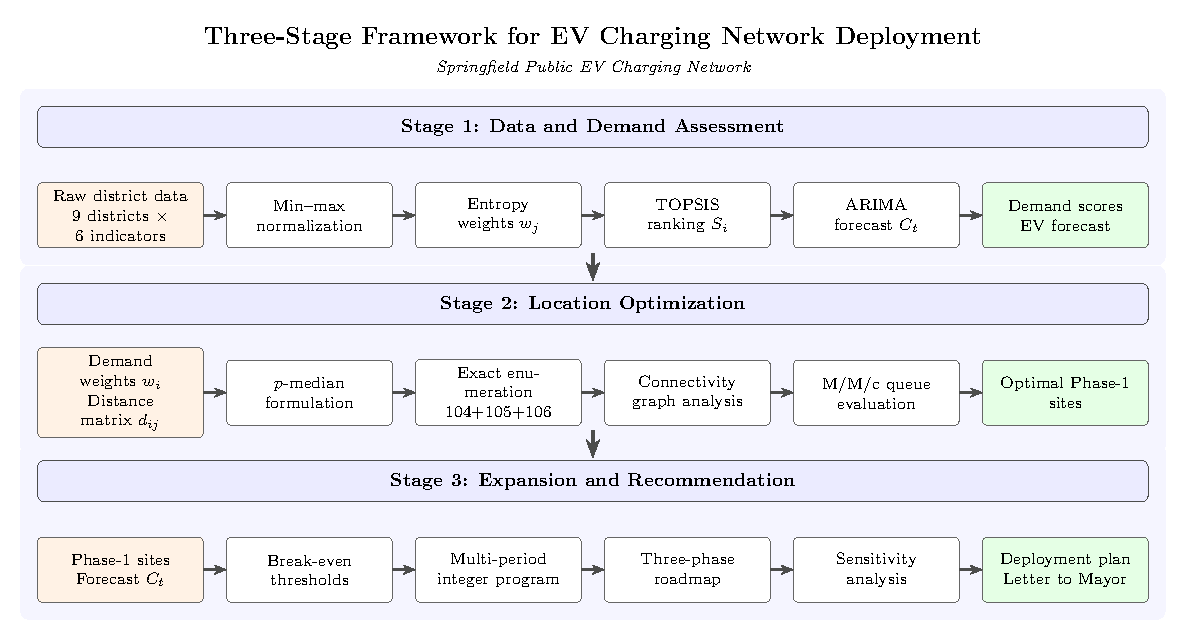
\includegraphics[width=\textwidth]{workflow.pdf}
\caption{Three-stage workflow of the deployment framework, from raw district data through demand assessment and location optimization to the final deployment plan and letter to the Mayor.}
\label{fig:workflow}
\end{figure}



% ============================================================
\section{Assumptions and Justification}
% ============================================================

We state our modeling assumptions explicitly and justify each one in turn. Assumptions are grouped by the stage of the model in which they arise.

\subsection{Demand and Forecasting Assumptions}

\textbf{Assumption 1:} Public charging demand is driven primarily by population, electric vehicle density, daily traffic volume, existing charger scarcity, and district type.

\textbf{Justification:} This assumption is supported both by the framing of the problem statement and by the empirical literature on charging-station utilization, which consistently finds that usage tracks local electric vehicle ownership, passing traffic, and the absence of home-charging alternatives. Commercial and administrative districts generate additional daytime demand from commuters and visitors, a phenomenon captured by the district-type indicator. These five drivers map directly to the six indicators used in the demand model.

\vspace{0.5em}
\textbf{Assumption 2:} Citywide electric vehicle adoption can be forecast from its own six-year history using an ARIMA time-series model, and the fleet cannot exceed a long-run ceiling of twenty-five thousand vehicles.

\textbf{Justification:} ARIMA is the natural choice when the only reliable predictor of the series is the series' own past, as it permits the data to determine the trajectory rather than imposing a fixed functional form. A pure ARIMA model possesses no saturation ceiling and would grow without bound over a long horizon; we therefore impose a conservative business bound of 25,000 vehicles. This bound sits well above the 2030 forecast and caps only the distant tail, leaving the near-term projections unchanged. A sensitivity sweep confirms that varying this ceiling between 20,000 and 30,000 vehicles does not affect the 2030 forecast or the phase-timing thresholds.



\subsection{Spatial and Feasibility Assumptions}

\textbf{Assumption 3:} The candidate sites listed in the problem data constitute the only feasible locations, and their reported costs and capacities are accurate.

\textbf{Justification:} Site-specific engineering constraints, such as electrical service availability and land suitability, are already reflected in the land-availability and maximum-capacity fields of the candidate data, so these reported values are the appropriate inputs to the location model.

\vspace{0.5em}
\textbf{Assumption 4:}A station serves demand in its own district and in nearby districts, with proximity captured by the supplied distance matrix, which is symmetric and represents driving distances between district centroids.



\textbf{Justification:} Drivers exhibit a strong preference for the nearest available charger, which is the reason our location model minimizes travel distance to the nearest station rather than ranking sites by abstract priority scores. The distance matrix is symmetric, consistent with road-network travel between district centers, and we use it both for the connectivity graph and for the p-median location model. We assume that district centroids adequately represent the spatial distribution of demand within each district.

\vspace{0.5em}
\textbf{Assumption 5:} The requirement to place at least one station in each of the nine districts is a terminal coverage goal rather than a constraint on first-phase selection.

\textbf{Justification:} The problem asks us to select four to six stations in Phase~1 while simultaneously requiring at least one station in each of nine districts; these requirements cannot hold together, because nine districts require at least nine stations. We resolve the conflict by treating per-district coverage as the goal of the complete three-phase rollout, achieved by Phase~3.

\subsection{Economic and Financial Assumptions}

\textbf{Assumption 6:} Each electric vehicle generates approximately fifty dollars per year in charging revenue, station installation is amortized over a ten-year horizon, and each public charger serves roughly seventy-five electric vehicles at full capacity.

\textbf{Justification:} These values anchor the break-even analysis. The revenue figure is a conservative industry average; the seventy-five-vehicle-per-charger rule sits within the range observed across comparable cities; and the ten-year amortization is standard in engineering economics.

\vspace{0.5em}
\textbf{Assumption 7:} In the supplementary queue evaluation, arrivals are Poisson, port-occupation times are exponentially distributed with mean one hour, and each electric vehicle makes one public-charging visit per week.

\textbf{Justification:} These are planning-level values used to compare layouts, not calibrated measurements. Poisson arrivals and exponential service times are the standard assumptions of the M/M/c queueing model and are appropriate for a first-order capacity check; the limitation is noted in Section~\ref{subsec:limitations}.

% ============================================================
\section{Variables and Notation}
\label{sec:notation}
% ============================================================

Table~\ref{tab:notation} collects the symbols used across the three models, grouped by the task in which they are introduced. Demand scores and weights are unitless, distances are in miles, and monetary amounts are in United States dollars.

\begin{table}[H]
\centering
\caption{Core notation used across the three modeling stages.}
\label{tab:notation}
\begin{tabular}{lll}
\toprule
Symbol & Meaning & Units \\
\midrule
$X = [x_{ij}]$ & decision matrix of raw indicator values & --- \\
$r_{ij}$ & min--max normalized indicator value & $[0,1]$ \\
$e_j, w_j$ & entropy and entropy weight of indicator $j$ & $[0,1]$ \\
$D_i^{+}, D_i^{-}$ & TOPSIS distances to ideal and negative-ideal solutions & --- \\
$S_i$ & demand priority score of district $i$ & 0--100 \\
$C_t$ & citywide electric vehicle registrations in year $t$ & vehicles \\
$w_i = S_i/100$ & demand weight used in the $p$-median model & $[0,1]$ \\
$d_{ij}$ & distance from district $i$ to site $j$ & miles \\
$y_j, x_{ij}$ & open-site and assignment binary variables & $\{0,1\}$ \\
$c_j, m_j$ & installation and annual maintenance cost of site $j$ & \$ \\
$L_j, M_j$ & land availability score and charger capacity of site $j$ & 1--5; chargers \\
$A_j$ & annualized cost of site $j$, equal to $0.1 c_j + m_j$ & \$/yr \\
$\mathrm{BE}_j$ & break-even electric vehicle count of site $j$ & vehicles \\
$\lambda_i(h)$ & arrival rate in district $i$ at hour $h$ & veh/hr \\
$\mu_i = 1/\tau_i$ & handling rate per charging port & veh/hr \\
$\rho_i$ & utilization, equal to $\lambda_i/(c_i\mu_i)$ & --- \\
$W_q$ & mean steady-state waiting time & hours \\
\bottomrule
\end{tabular}
\end{table}

% ============================================================
\section{Task 1: Charging Demand Assessment}
% ============================================================

\subsection{Data Exploration and Preprocessing}

Before constructing any model, we examine the raw dataset for quality and structure, confirming that the data support the assumptions that follow and flagging values that would distort the analysis. Every cell of the district indicator matrix and candidate-site table is present, so no imputation is required. For each indicator we compute standardized $Z$-scores and flag any district with $|Z| > 2.5$. Exactly one district qualifies: Downtown's electric vehicle density, at 4.94\%, sits more than two standard deviations above the mean. This is a genuine feature of the data rather than a measurement error, and it is the principal reason Downtown leads the demand ranking that follows.

We also compute the pairwise correlation matrix of the six indicators and flag coefficients with magnitude above 0.8. As shown in Figure \ref{fig:corr}, four pairs exceed this threshold, led by daily traffic and district type with $r = 0.92$. The entropy-weight method employed below handles this redundancy by down-weighting correlated indicators, so no manual removal is necessary.

\begin{figure}[H]
\centering
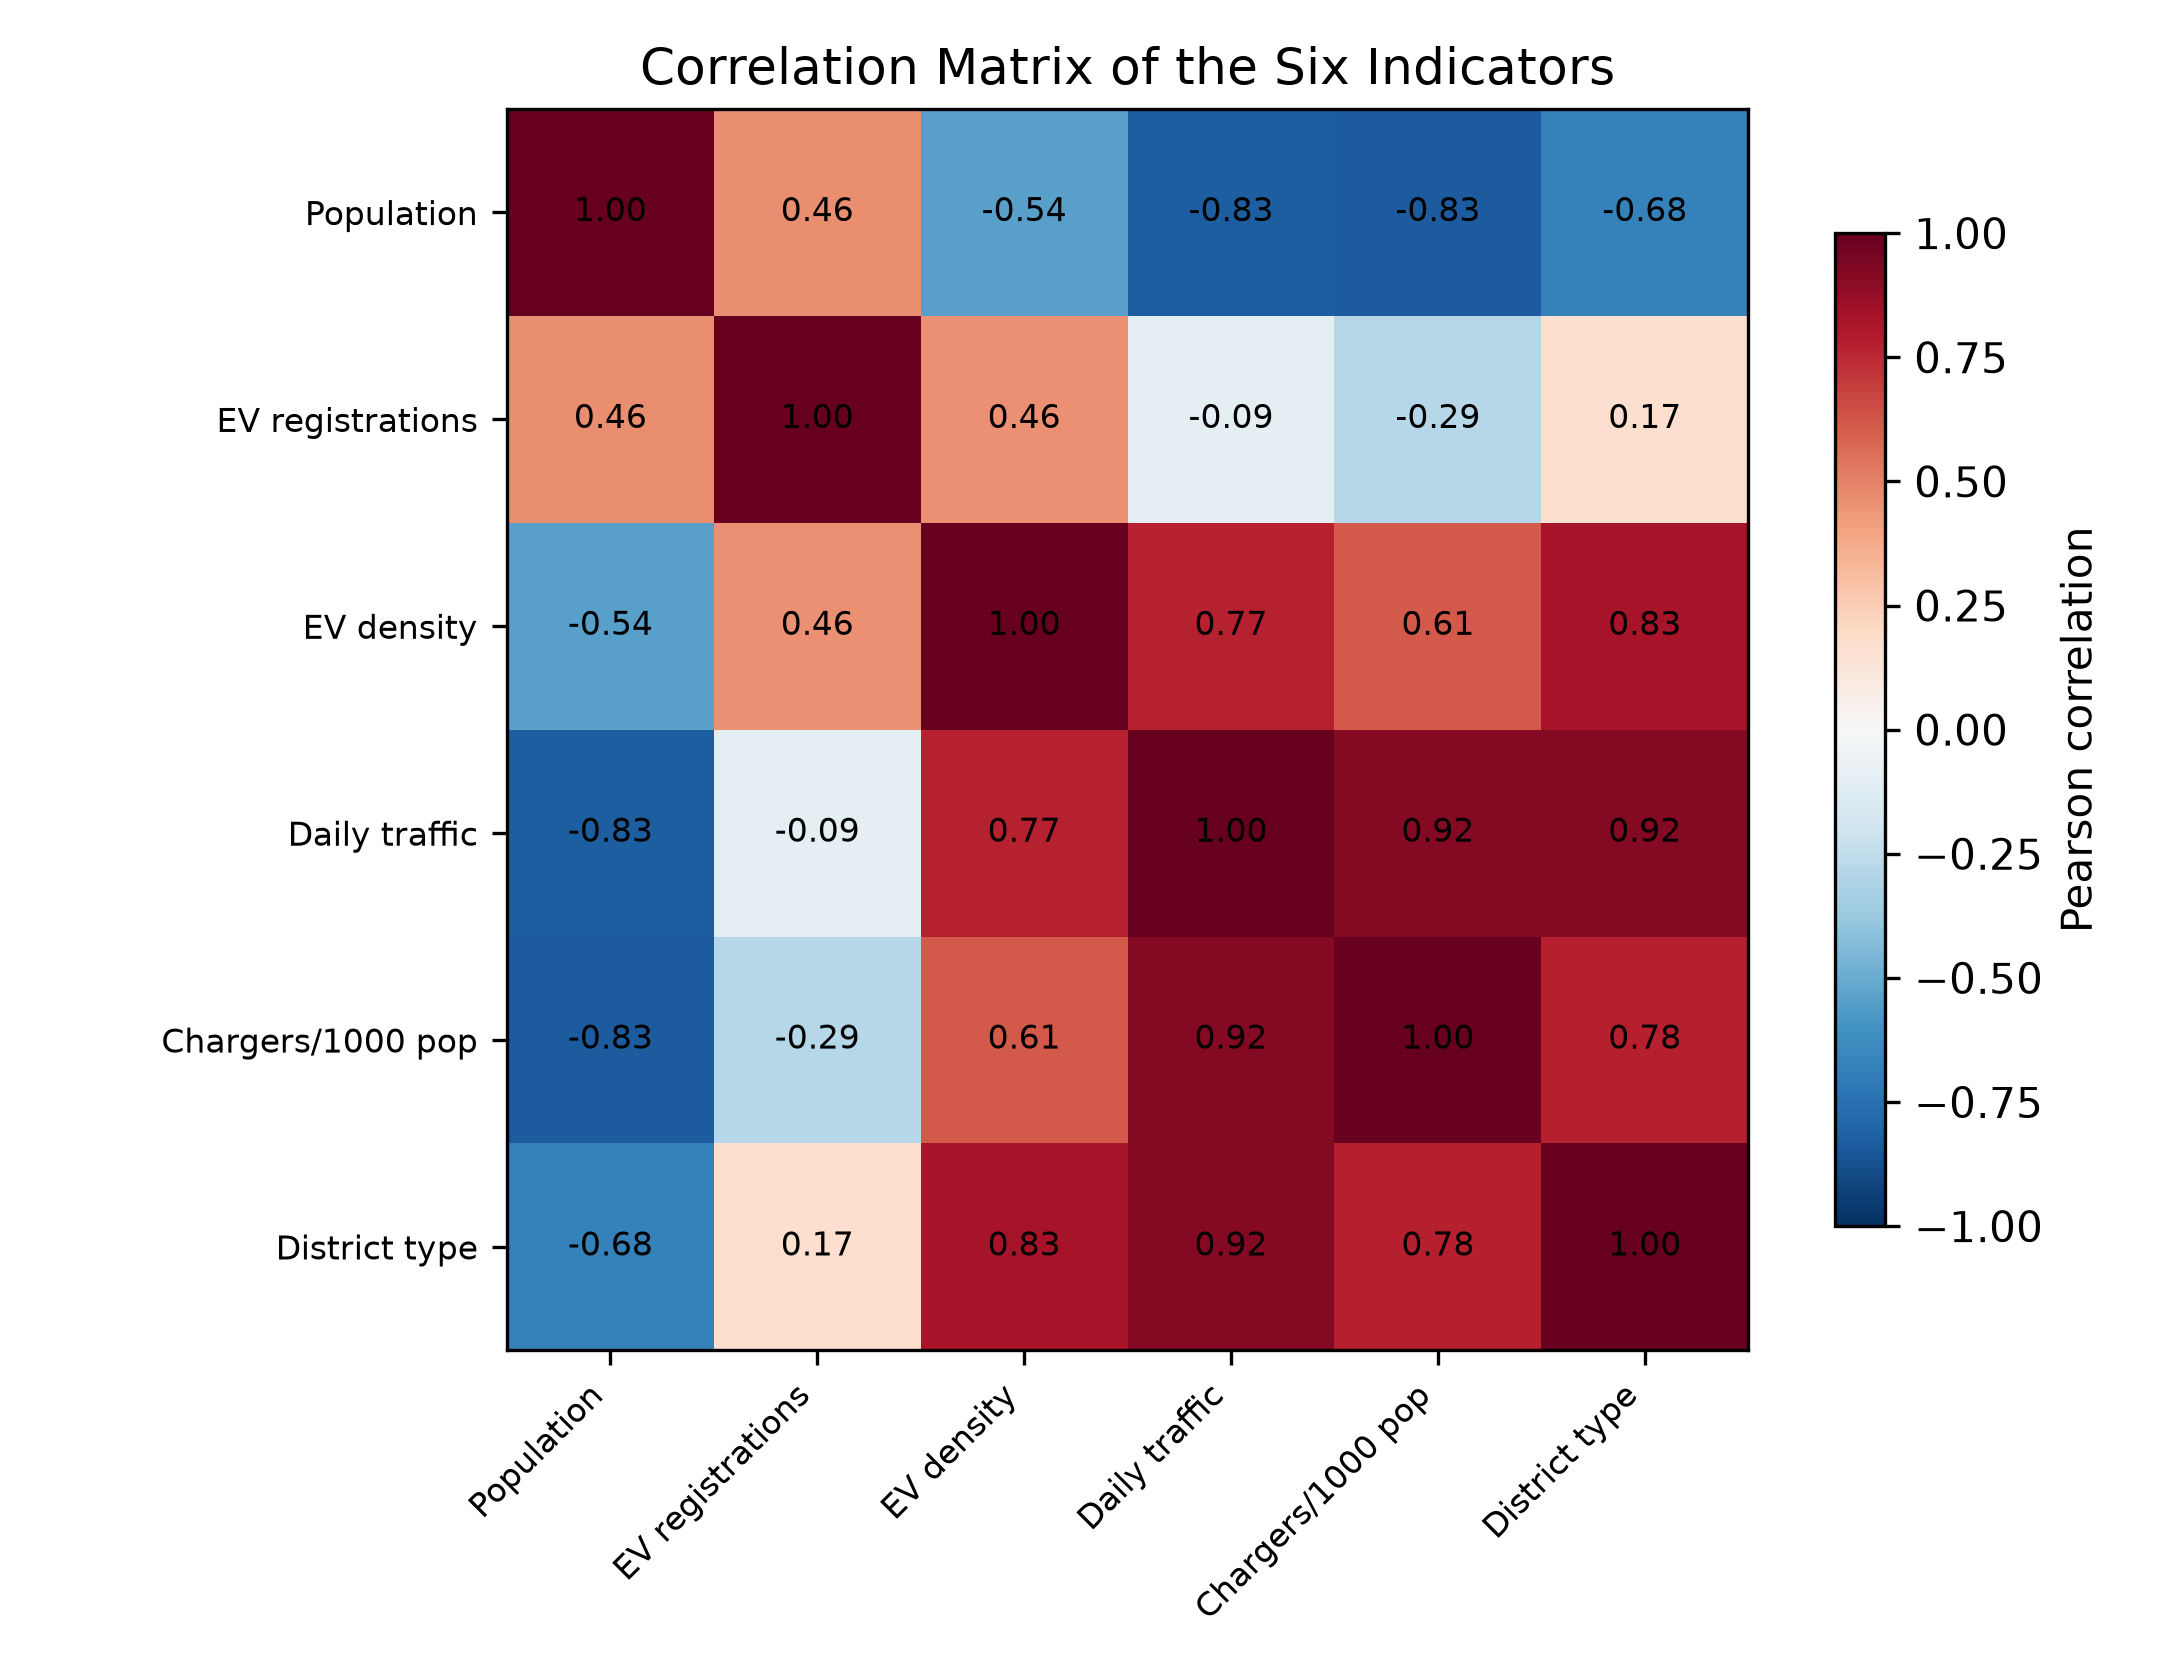
\includegraphics[width=0.7\textwidth]{ev_correlation.png}
\caption{Pairwise correlation matrix of the six demand indicators. Color encodes the Pearson coefficient from $-1$ to $+1$.}
\label{fig:corr}
\end{figure}

\subsection{Factors Influencing Charging Demand}

We identify five primary drivers of public charging demand, each of which enters our evaluation model as a measurable indicator.

\begin{addmargin}[1.5em]{0em}

\textbf{Population.} A larger resident population supports a larger potential electric vehicle base, as it corresponds to a larger pool of potential adopters.

\textbf{Electric vehicle density.} Many electric vehicles per resident produce an immediate, localized demand for charging, whereas the same number of vehicles spread thinly across a large population exerts lower pressure on any specific location.

\textbf{Daily traffic volume.} Daily traffic captures through-flow and visitor activity that resident population alone misses. A busy commercial corridor requires charging capacity for non-residents even when few electric vehicles are registered locally, a phenomenon evident in the Mall District, which possesses a small resident population but heavy traffic.

\textbf{Existing charger scarcity.} Demand for new public charging is highest where supply is thinnest, measured as the number of existing chargers per thousand residents. This indicator identifies districts in which supply has failed to keep pace with adoption.

\textbf{District type.} Commercial, administrative, and educational districts generate daytime and visitor demand that residential districts do not, so we map each district type to a propensity score that encodes its expected charging intensity.

\end{addmargin}

\subsection{Evaluation Indicator System and Entropy Weights}
\label{subsec:entropy}

We formalize these factors into six indicators for the nine districts. All indicators are oriented as benefit-type, meaning that a higher value raises demand priority. We apply min--max normalization to each indicator, then compute Shannon entropy to derive objective weights. Indicators on which districts differ sharply carry more information for ranking, and consequently receive larger weights; indicators on which districts score similarly carry less discriminating information and receive smaller weights.

\begin{table}[H]
\centering
\caption{Entropy weights for the six demand indicators.}
\label{tab:weights}
\begin{tabular}{lccc}
\toprule
Indicator & Direction & Entropy $e_j$ & Weight $w_j$ \\
\midrule
I1 Population & $+$ & 0.887 & 0.152 \\
I2 Electric vehicle registrations & $+$ & 0.863 & 0.185 \\
I3 Electric vehicle density & $+$ & 0.846 & 0.208 \\
I4 Daily traffic volume & $+$ & 0.866 & 0.181 \\
I5 Chargers per 1{,}000 residents & $-$ & 0.934 & 0.089 \\
I6 District type propensity & $+$ & 0.863 & 0.185 \\
\bottomrule
\end{tabular}
\end{table}

The resulting weights reveal a clear hierarchy. Electric vehicle density, electric vehicle registrations, daily traffic, and district type receive nearly equal weights between 0.18 and 0.21, together accounting for approximately seventy-six percent of the total. These four factors discriminate best among the districts, which is why the data-driven weighting elevates them. Charger scarcity receives the smallest weight, at 0.089, because most districts possess similarly low charger counts and the indicator therefore offers little separation. Population occupies an intermediate position, because large residential districts do not translate one-to-one into public charging demand.

\subsection{TOPSIS Ranking and Demand Priority Scores}

The entropy-weight method produces a weight for each indicator, but weights alone do not rank districts. To convert weights into a district-level score, we use TOPSIS rather than a weighted sum, because a weighted sum allows a strong score on one indicator to offset weak scores on others, whereas TOPSIS penalizes districts that lag on any dimension. 

We rank districts using the Technique for Order Preference by Similarity to Ideal Solution. The method constructs a weighted decision matrix, defines an ideal solution and a negative-ideal solution, and measures each district's Euclidean distance to both. The demand priority score is defined as the ratio of the distance to the negative-ideal solution over the sum of both distances, rescaled to a 0--100 range.

\begin{table}[H]
\centering
\caption{Charging demand priority scores and rankings.}
\label{tab:demand}
\begin{tabular}{clccc}
\toprule
Rank & District & $D^{+}$ & $D^{-}$ & Score \\
\midrule
1 & Downtown      & 0.143 & 0.372 & 72.24 \\
2 & Eastside      & 0.205 & 0.239 & 53.80 \\
3 & Mall District & 0.269 & 0.272 & 50.30 \\
4 & University    & 0.234 & 0.206 & 46.80 \\
5 & Southside     & 0.271 & 0.220 & 44.75 \\
6 & Northside     & 0.278 & 0.200 & 41.88 \\
7 & Westside      & 0.293 & 0.200 & 40.58 \\
8 & Industrial    & 0.292 & 0.160 & 35.46 \\
9 & Riverside     & 0.374 & 0.132 & 26.11 \\
\bottomrule
\end{tabular}
\end{table}

Downtown leads by a substantial margin, its score of 72.24 reflecting the combination of high electric vehicle density, heavy traffic, and commercial district classification. The middle tier---Mall District through Westside---spans approximately ten points, indicating that these districts are broadly comparable in demand. Riverside ranks last at 26.11 despite possessing no public chargers whatsoever; its scarcity is a future opportunity rather than a current bottleneck, a distinction whose implications become clear in the location analysis of Section \ref{sec:location}.

\subsection{Citywide Electric Vehicle Registration Forecast}
\label{subsec:forecast}

To plan network expansion, we must forecast how many electric vehicles Springfield will contain in the coming years. The city holds only six years of registration data, and the series is non-stationary, so a regression on a time index is unreliable. We model the series with a classical ARIMA process and retain a logistic S-curve as a technology-diffusion comparison baseline. The two methods serve complementary purposes: ARIMA lets the recent trend determine the trajectory without imposing a fixed shape, while the logistic curve reflects standard diffusion theory and provides an optimistic upper bound against which the ARIMA forecast can be checked.

We first choose the integration order using the Augmented Dickey--Fuller test. The test fails to reject a unit root in both the level and the first difference, so we treat the series as integrated of order two and set $d = 2$. Let $C_t$ denote citywide registrations in year $t$ and $\nabla^d C_t$ its $d$-th difference. The general ARIMA$(p,d,q)$ model is
\begin{equation}
\nabla^d C_t = \phi_1 \nabla^d C_{t-1} + \cdots + \phi_p \nabla^d C_{t-p} + \epsilon_t + \theta_1 \epsilon_{t-1} + \cdots + \theta_q \epsilon_{t-q},
\end{equation}
where $\epsilon_t$ is white noise. Selecting $p, q \in \{0,1\}$ by minimum AIC yields ARIMA$(1,2,0)$ with $\hat{\phi}_1 = 0.935$, AIC $= 52.07$, and residual standard deviation of seventy-nine vehicles. The second-differenced series and its autocorrelation and partial autocorrelation functions appear in Figure~\ref{fig:acf}. Because only four second-differenced observations are available, partial autocorrelations can be estimated at lag one only; both lag-one values fall within the 95\% significance bounds, which is consistent with the ARIMA$(1,2,0)$ specification though not strong evidence for it. Diagnostics possess limited power on such a short series, a limitation noted in Section~\ref{subsec:limitations}.

\begin{figure}[H]
\centering
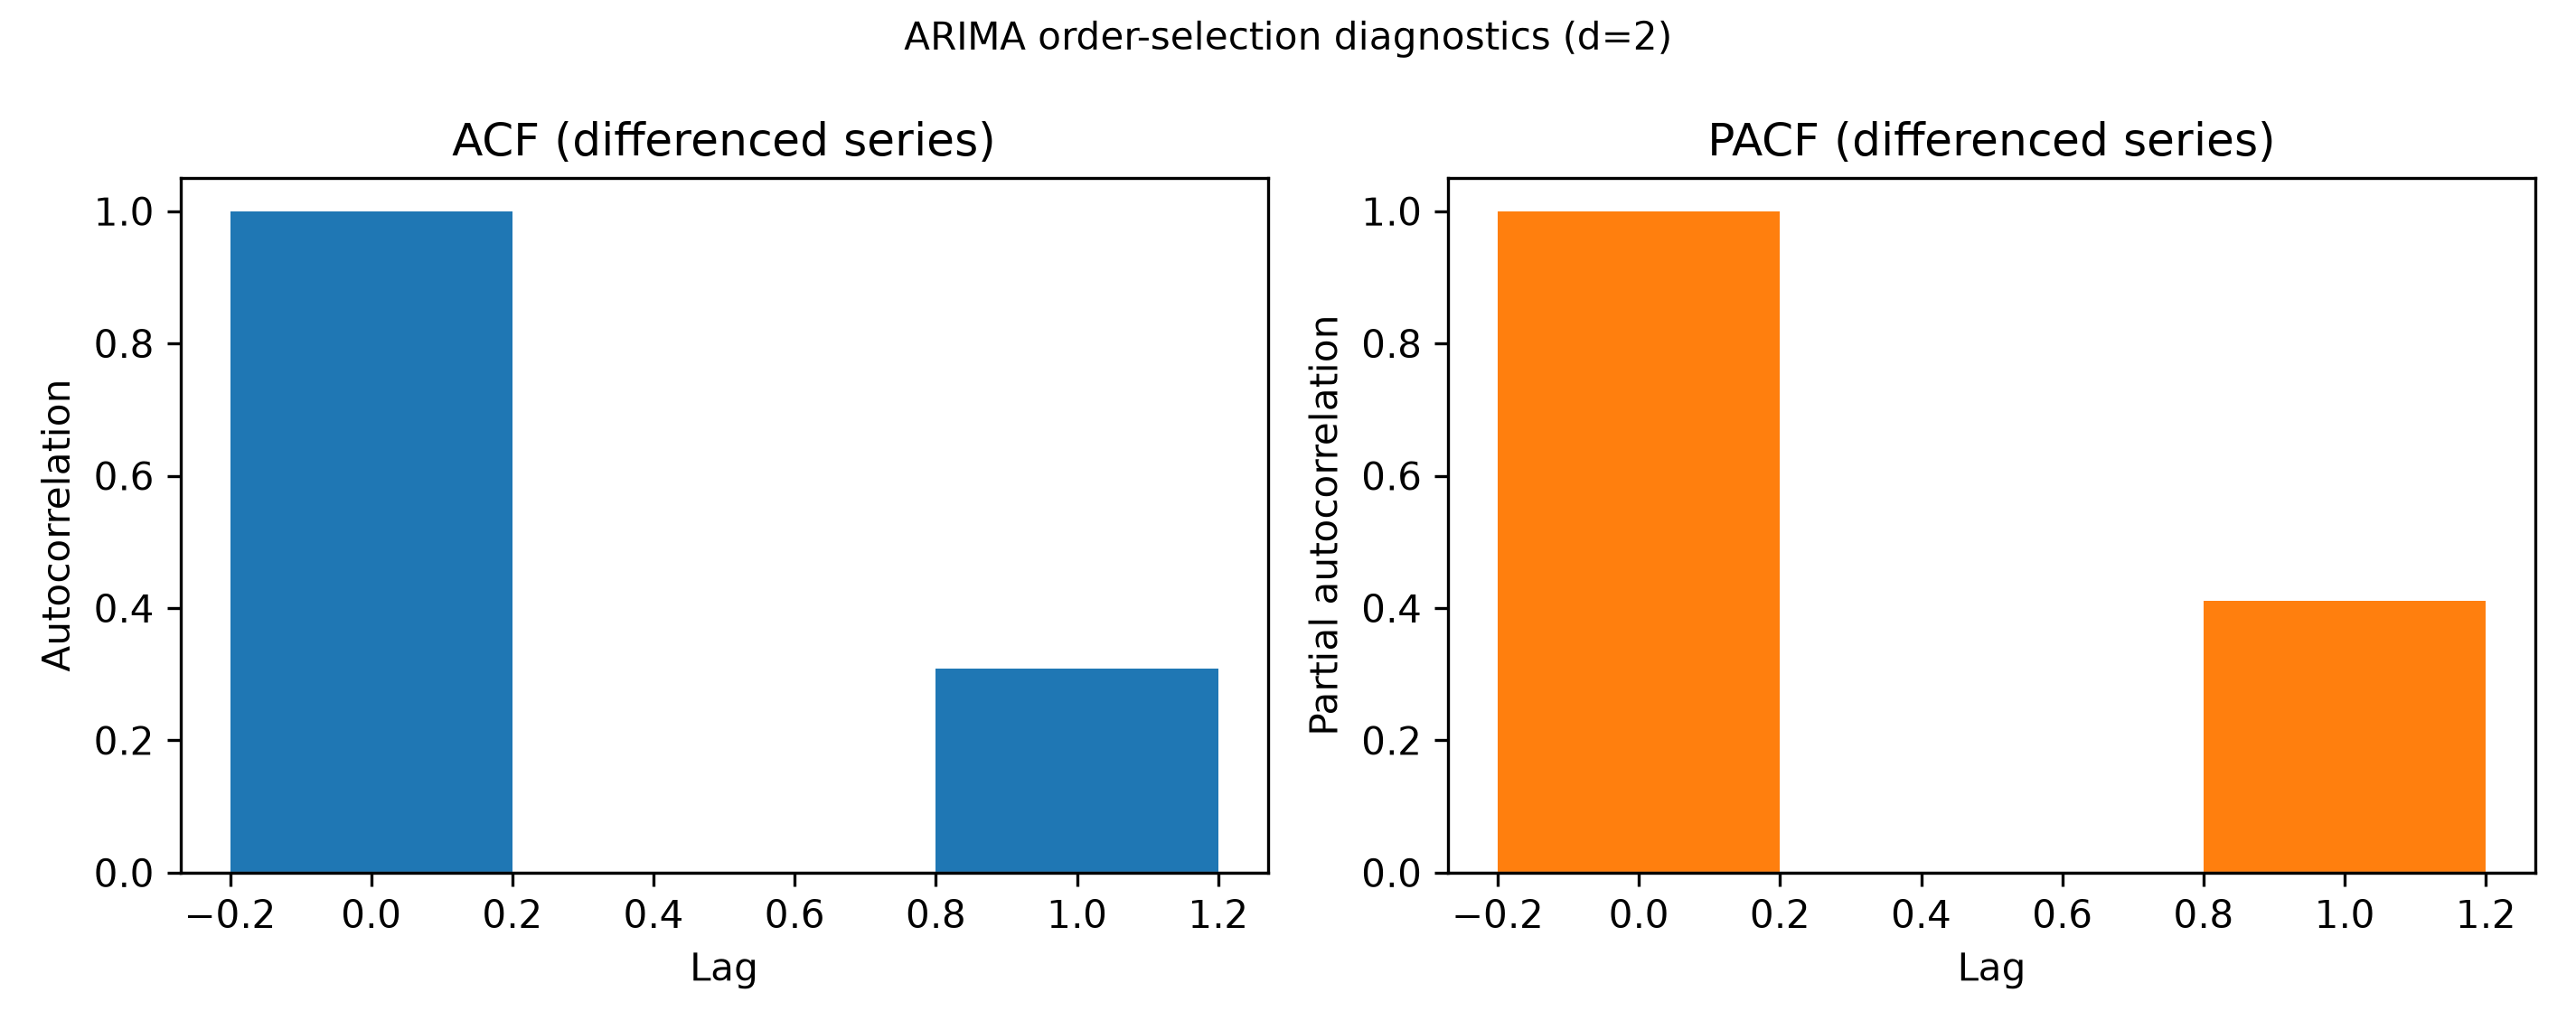
\includegraphics[width=0.8\textwidth]{ev_arima_acf_pacf.png}
\caption{Second-differenced electric vehicle registration series with its autocorrelation and partial autocorrelation functions.}
\label{fig:acf}
\end{figure}

A pure ARIMA model has no saturation ceiling, so we impose a conservative business upper bound of 25{,}000 vehicles, well above the 2030 forecast. This cap binds only the distant tail and does not affect the near-term projections.

The logistic model is the classic technology-diffusion curve, assuming that growth begins slowly, accelerates, and eventually saturates at a carrying capacity $K$. Fitting this curve to the same data provides a useful upper-bound scenario. We do not adopt it as the primary forecast, because the short series shows no clear evidence of saturation and the imposed S-shape may overstate long-run growth.

\begin{table}[H]
\centering
\caption{Electric vehicle registration forecast: ARIMA versus logistic baseline.}
\label{tab:forecast}
\begin{tabular}{lcccc}
\toprule
Model & 2025 & 2026 & 2027 & 2030 \\
\midrule
Logistic (baseline) & 3{,}228 & 4{,}734 & 6{,}725 & 14{,}751 \\
ARIMA (primary)     & 3{,}242 & 4{,}548 & 6{,}083 & 11{,}915 \\
\bottomrule
\end{tabular}
\end{table}

\begin{figure}[H]
\centering
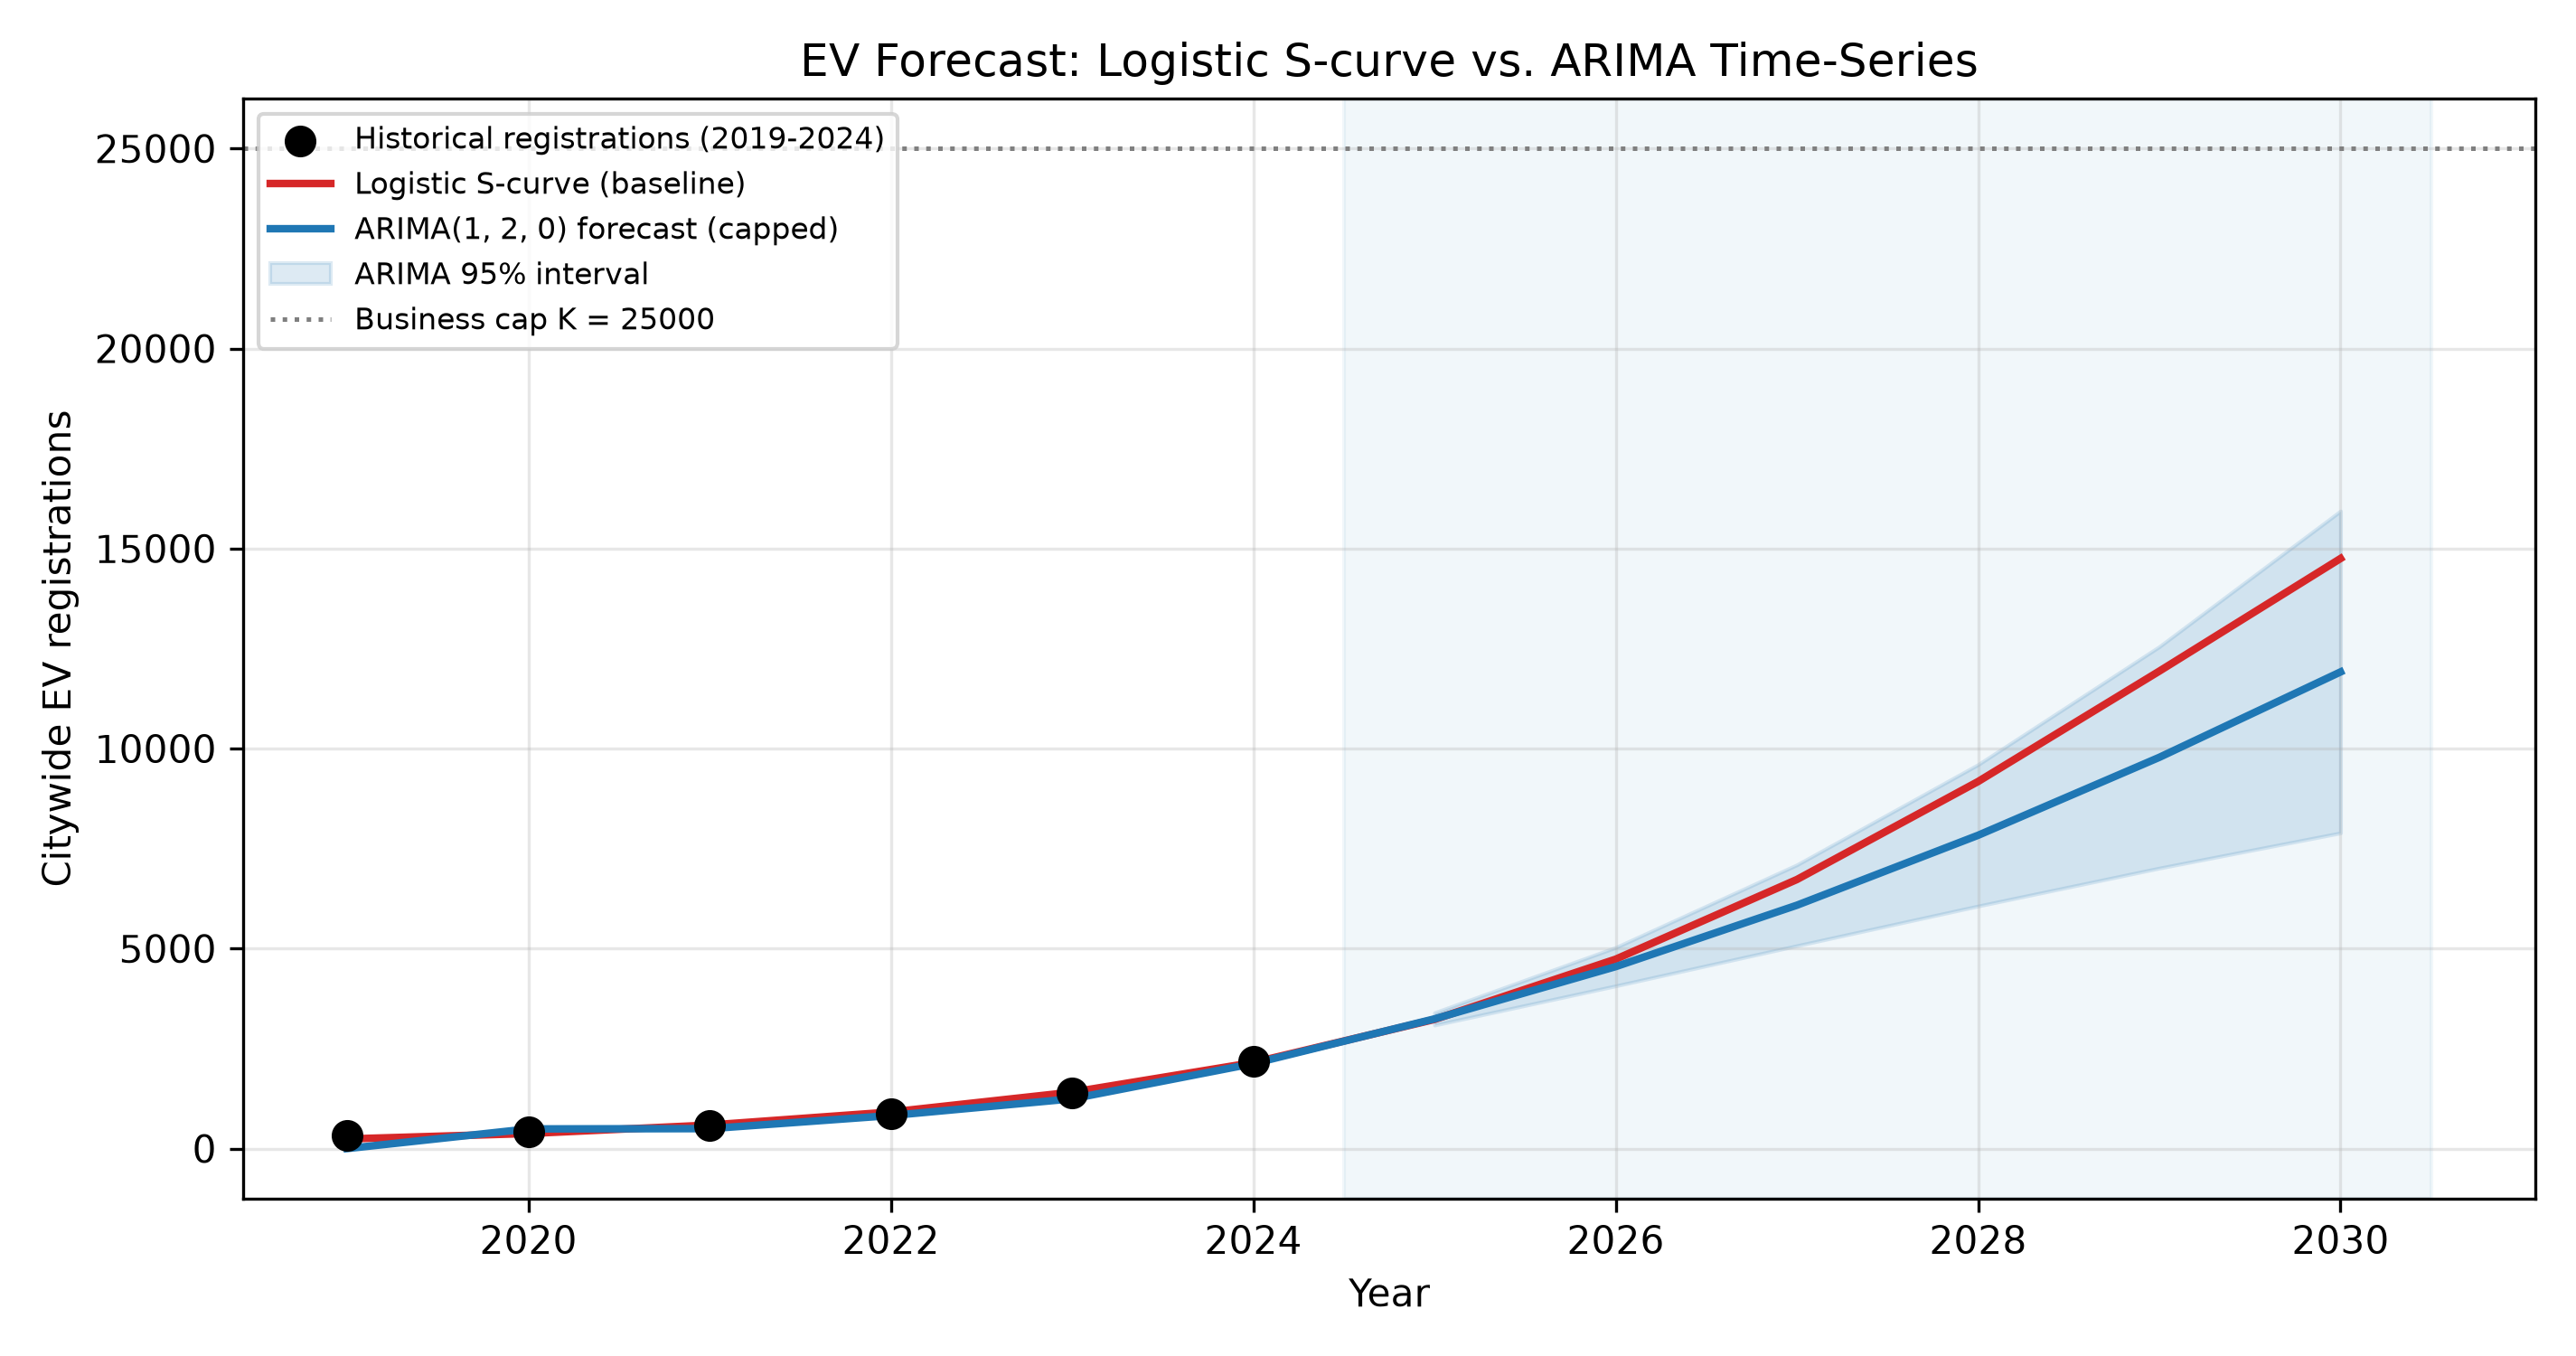
\includegraphics[width=0.8\textwidth]{ev_forecast_compare.png}
\caption{Citywide electric vehicle forecast. Black points are historical registrations. The blue curve is the ARIMA$(1,2,0)$ forecast with its 95\% interval; the red curve is the logistic S-curve baseline.}
\label{fig:forecast}
\end{figure}

The two forecasts agree closely through 2026 and diverge thereafter. The logistic curve, forced to follow an S-shape, inflects near 2029 and reaches 14{,}751 by 2030; the ARIMA model, constrained only by the 25{,}000 cap, reaches 11{,}915. Both forecasts cross the phase-trigger thresholds derived in Section~6 in the same years, so the timing of deployment phases is insensitive to the choice of method. We adopt ARIMA as the primary forecast for three reasons. Its residuals satisfy the assumptions of statistical inference. It follows the recent growth trend without forcing an early inflection, making it more conservative for public investment. And the two models produce similar near-term forecasts through 2027, so the early phases of the roadmap are robust to the choice.

\subsection{Arrival Rate Profiles}
\label{subsec:peak}

To supplement the static demand score with a service-layer evaluation, we convert district electric vehicle counts into hourly arrival rates. Each electric vehicle generates one public-charging visit per week. We split daily arrivals into a four-hour peak, during which forty percent of visits occur, and a twenty-hour off-peak period during which the remaining sixty percent occur. For a district with $E$ registered electric vehicles, the peak arrival rate is
\[
\lambda_{\text{peak}} = \frac{0.4 \cdot (E/7)}{4} = \frac{E}{70}\ \text{vehicles per hour},
\]
and the off-peak rate is
\[
\lambda_{\text{off}} = \frac{0.6 \cdot (E/7)}{20} \approx \frac{E}{233}\ \text{vehicles per hour}.
\]

Applying these peak and off-peak arrival rates to each district yields the profile shown in Figure~\ref{fig:peak}. The resulting curves separate cleanly by district type. Commercial and administrative districts, led by Downtown and the Mall District, peak between 07:00 and 22:00, reflecting commuter and visitor activity. Residential districts such as Northside, Westside, and Riverside peak sharply between 16:00 and 20:00, when residents return home. University shows a narrow morning surge, Industrial a long plateau from 07:00 to 23:00, and the two mixed districts, Southside and Eastside, blend both patterns. This heterogeneity matters because a single citywide peak would overstate the load in commercial districts and understate it in residential ones. The district-specific profiles are therefore used directly as the peak arrival rates $\lambda_i$ in Section~\ref{sec:service}.

\begin{figure}[H]
\centering
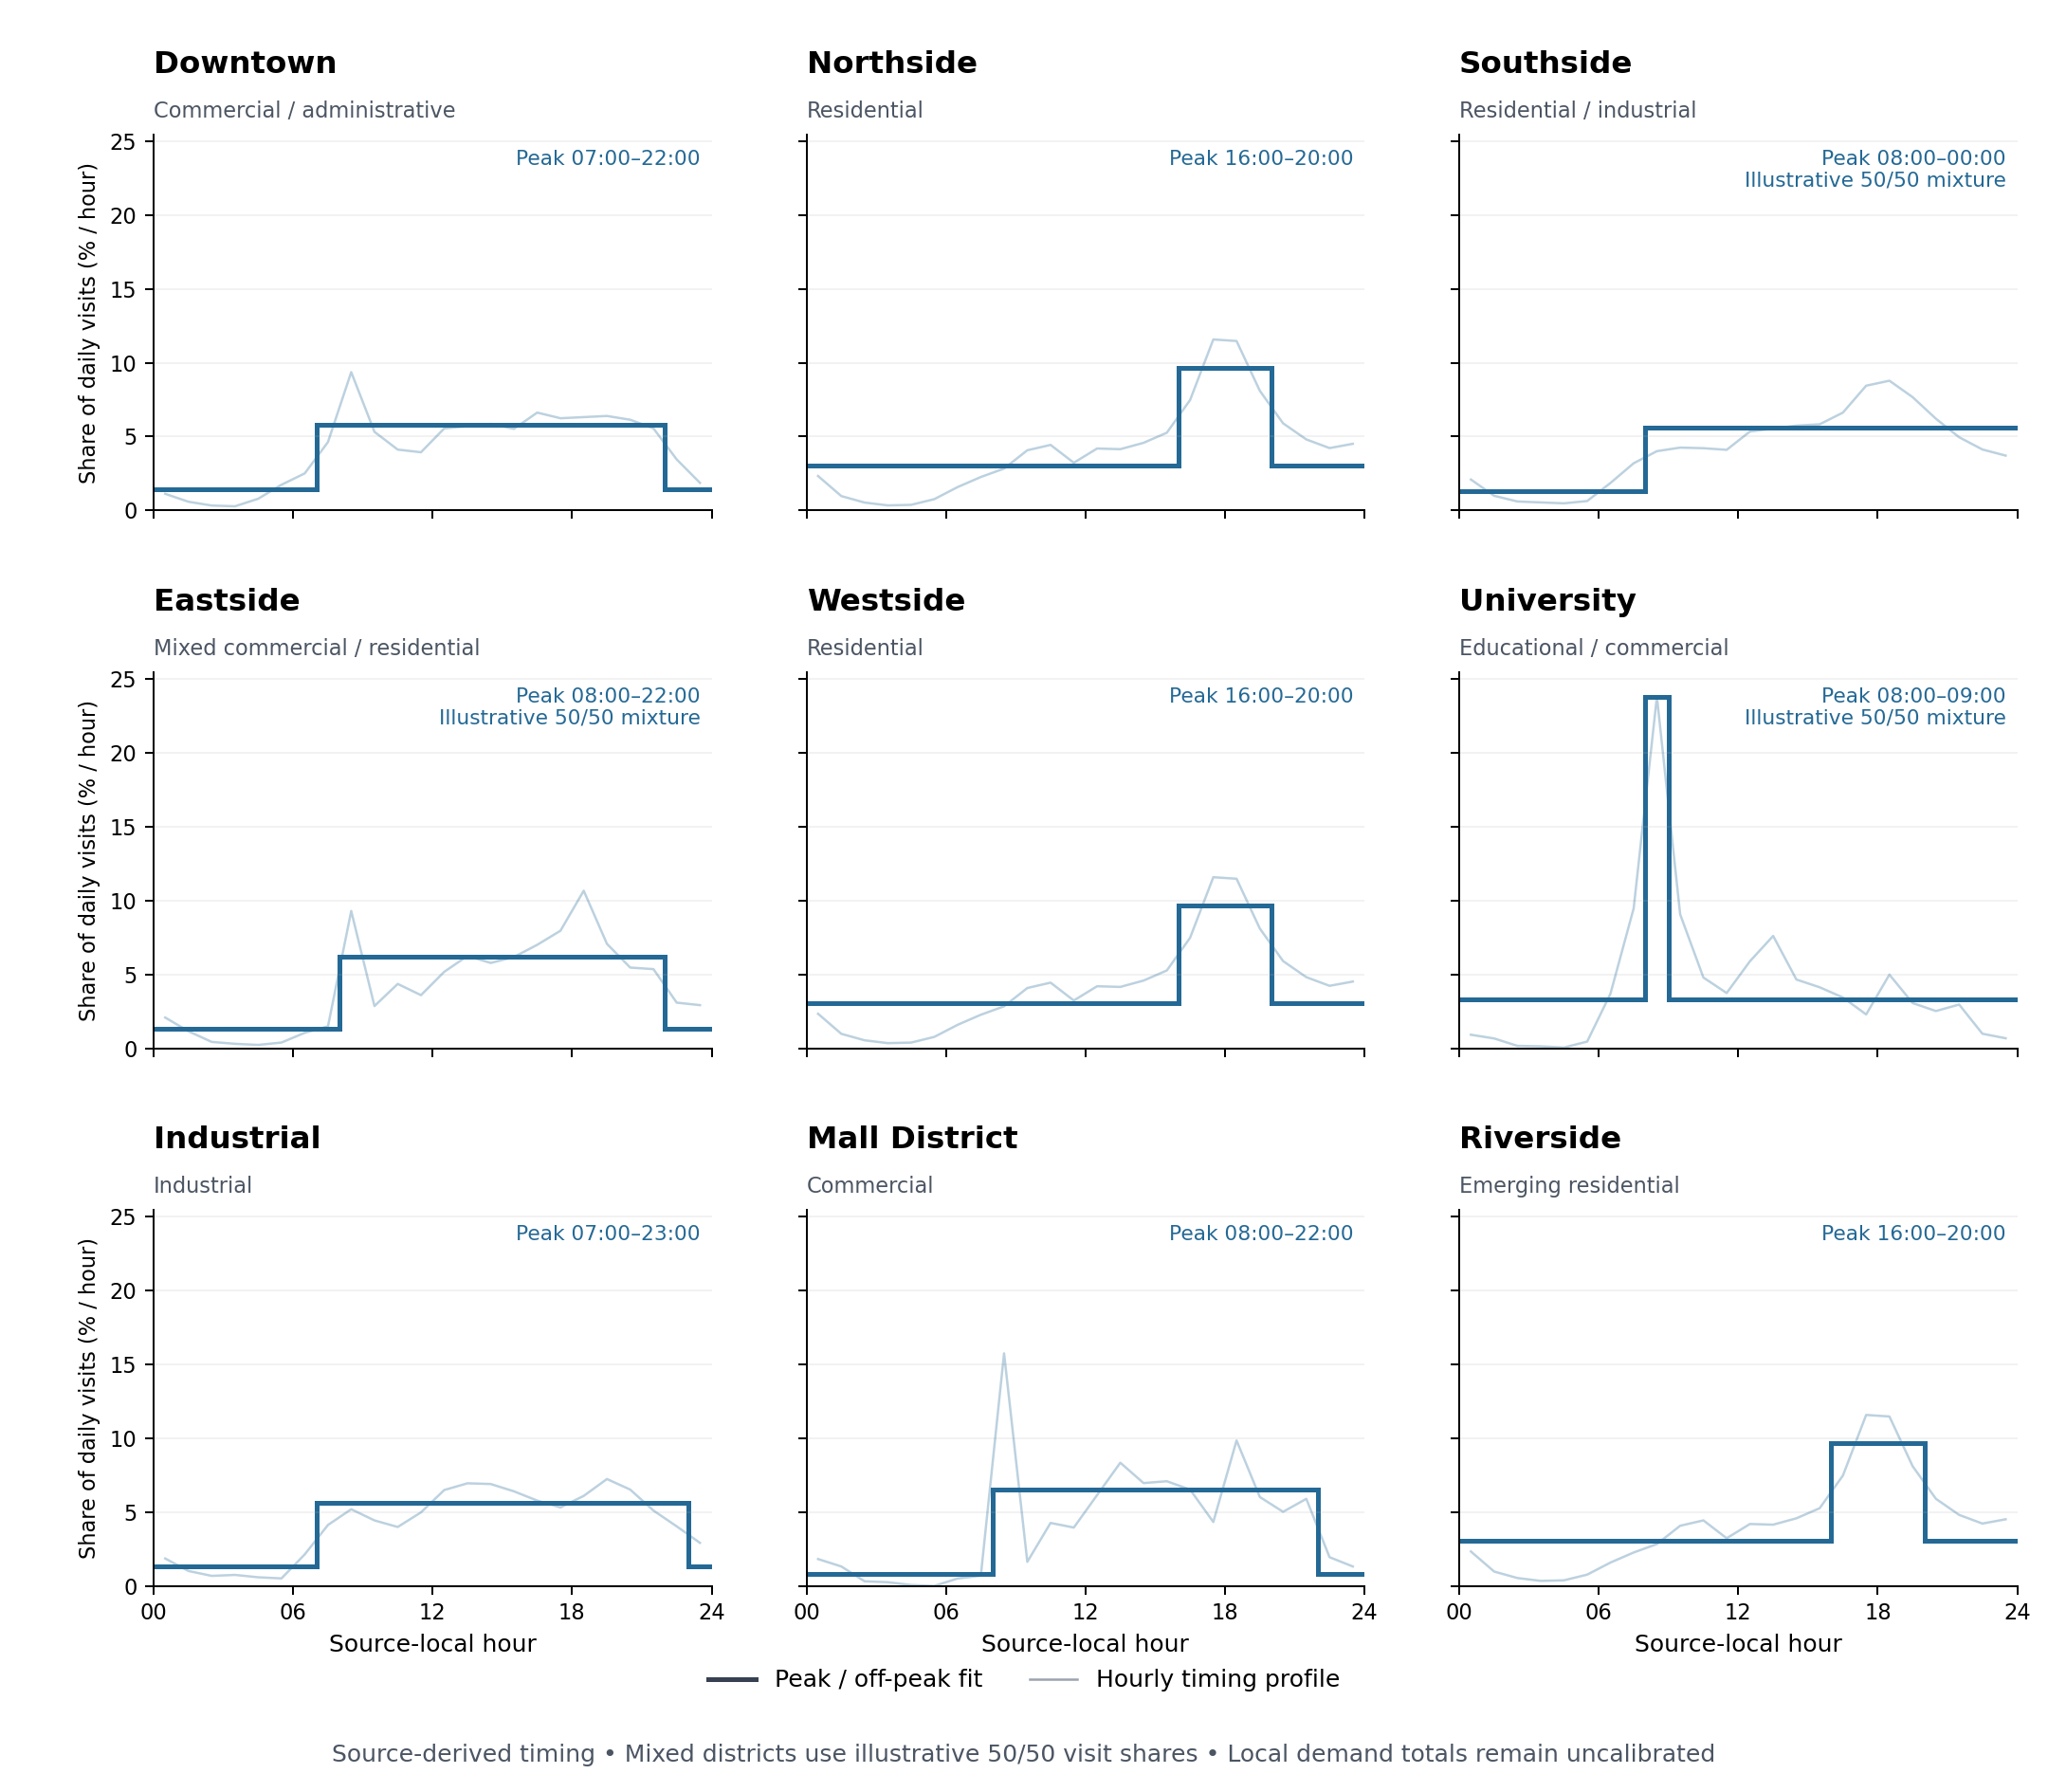
\includegraphics[width=0.85\textwidth]{ev_district_peak_profiles.png}
\caption{Peak and off-peak arrival profiles by district.}
\label{fig:peak}
\end{figure}

Finally, the queue parameters established here also justify the utilization rule used for phase timing in Section~\ref{sec:breakeven}. A charger with a mean service time of one hour, operating at a planned utilization of forty-five percent, completes approximately $24 \times 0.45 = 10.8$ sessions per day, or roughly seventy-five sessions per week. Since each electric vehicle generates one public-charging visit per week, this implies that one charger serves approximately seventy-five electric vehicles at steady state. This figure sits within the EV-to-charger ratios reported for mid-size cities \cite{funke2019} and is adopted as the planning midpoint for the citywide phase-trigger thresholds in Section~\ref{sec:breakeven}.

% ============================================================
\section{Task 2: Location Optimization}
\label{sec:location}
% ============================================================

\subsection{Site Attributes and the Facility-Location Objective}

A charging station is useful only if drivers can reach it, so our location model minimizes the distance from each district to its closest station rather than a sum of priority scores attached to sites. We weight that distance by district demand, since a mile of extra travel matters more where many electric vehicles are registered than where few are.

Each district $i$ carries demand weight $w_i = S_i/100$, the TOPSIS score of Section \ref{sec:notation} rescaled to the unit interval. A station in district $j$ serves every district within the five-mile coverage radius, the same threshold used in the connectivity analysis of Section \ref{subsec:forecast}, so both share one distance standard. A layout's cost is the sum over districts of $w_i$ times the distance to the nearest station. This is the demand-weighted travel distance, which the model minimizes.

\subsection{$p$-Median Facility-Location Formulation}

We formalize the objective as a $p$-median facility-location problem. Let $y_j \in \{0,1\}$ indicate whether site $j$ is opened, and let $x_{ij} \in \{0,1\}$ indicate whether district $i$ is assigned to the station at site $j$. The model chooses open sites and assigns every district to one open site so as to minimize the demand-weighted travel distance:

\begin{equation}
\min \sum_{i=1}^{9}\sum_{j=1}^{10} w_i \, d_{ij} \, x_{ij}
\end{equation}

subject to

\begin{align}
  & \hspace{1.5cm} \sum_{j=1}^{10} x_{ij} = 1, \quad i = 1,\ldots,9 && \text{(every district served)} \\[3pt]
  & \hspace{1.5cm} x_{ij} \le y_j, \quad \forall i,j && \text{(only open stations serve)} \\[3pt]
  & \hspace{1.5cm} x_{ij} = 0 \;\; \text{whenever } d_{ij} > 5 && \text{(coverage radius)} \\[3pt]
  & \hspace{1.5cm} \sum_{j=1}^{10} c_j \, y_j \le 200 && \text{(budget)} \\[3pt]
  & \hspace{1.5cm} 4 \;\le\; \sum_{j=1}^{10} y_j \le 6 && \text{(station count)} \\[3pt]
  & \hspace{1.5cm} L_j \ge 3 y_j, \quad M_j \ge 4 y_j && \text{(land and capacity filters)} \\[3pt]
  & \hspace{1.5cm} y_j, x_{ij} \in \{0,1\} && \text{(binary decision variables)}
\end{align}

The first three constraints define the assignment. The coverage radius sets $x_{ij} = 0$ when district $i$ lies more than five miles from site $j$. Because drivers always choose the nearest station, each district is assigned to its closest open site in the optimal solution, so we solve the model by enumerating the open sets directly.

We choose a $p$-median objective over a maximal-covering one because maximal covering ignores distance within the radius. Given the five-mile radius and the compactness of the districts, a few central stations already cover the city, so maximal covering ceases to discriminate beyond roughly three stations, whereas the $p$-median objective continues to reward smaller distances after coverage is met.

Maintenance cost and break-even are deliberately excluded from the objective: they depend on charger utilization, a system-wide quantity rather than a site-level one, so embedding them in site selection would double-count economics and dilute the spatial logic. The economic layer is applied after selection in Section~\ref{sec:service}.

The feasible sets number $\binom{10}{4} + \binom{10}{5} + \binom{10}{6} = 672$, so we enumerate every combination, evaluate its demand-weighted distance, and retain the smallest, breaking ties by lower cost. The result is provably optimal.

\subsection{Optimal Phase-1 Selection}

The enumeration returns the optimum in Table~\ref{tab:phase1}.

\begin{table}[H]
\centering
\caption{Optimal Phase-1 station selection.}
\label{tab:phase1}
\begin{tabular}{llcccc}
\toprule
Site & District & $w_i$ & Install cost & Land & Max chargers \\
\midrule
S2 & Downtown   & 0.7224 & \$380{,}000 & 4 &  8 \\
S3 & Northside  & 0.4188 & \$300{,}000 & 5 &  6 \\
S4 & Southside  & 0.4475 & \$280{,}000 & 4 &  6 \\
S5 & Eastside   & 0.5380 & \$320{,}000 & 5 &  6 \\
S6 & Westside   & 0.4058 & \$250{,}000 & 5 &  4 \\
S8 & Industrial & 0.3546 & \$400{,}000 & 4 & 10 \\
\midrule
\multicolumn{2}{l}{\textbf{Total}} & & \textbf{\$1{,}930{,}000} & & \textbf{40} \\
\bottomrule
\end{tabular}
\end{table}

The $p$-median optimum selects six stations across six distinct districts at \$1.93 million, leaving the demand-weighted travel distance at 3.35 miles. It does not double up in Downtown, since a second station there saves no travel distance once S2 already serves the district at zero miles.

The most instructive choice is S8 (Industrial). Industrial ranks only eighth in demand at 0.3546, yet it is selected ahead of the Mall District (0.5030) and University (0.4680) because of distance: its only neighbor within five miles is Southside, so without its own station its drivers face a 3.5-mile drive, while the Mall District and University already lie within two miles of a Phase-1 station.

\subsection{Comparison Against Naive Strategies}

We verify that the $p$-median layout earns its complexity by comparing it against three naive placement rules that a planner might apply by hand. Each rule opens six stations, and each is scored by the same demand-weighted distance, so the comparison is directly interpretable.

\begin{table}[H]
\centering
\caption{Phase-1 placement: $p$-median versus naive strategies.}
\label{tab:naive}
\begin{tabular}{llcc}
\toprule
Strategy & Selected sites & Distance & Improvement \\
\midrule
$p$-median & S2, S3, S4, S5, S6, S8 & 3.35 & --- \\
Demand-greedy & S2, S3, S4, S5, S6, S7 & 3.42 & 2.1\% \\
Population-split & S3, S4, S5, S6, S7, S10 & 4.05 & 17.3\% \\
Random (mean of 2{,}000) & --- & 4.82 & 30.5\% \\
\bottomrule
\end{tabular}
\end{table}

The $p$-median layout beats the demand-greedy rule by only 2.1\%, because a demand ranking and a distance ranking agree on most sites. It beats the population-based rule by 17.3\% and a random placement by 30.5\% on average. The gains are concentrated where the two rankings disagree: the $p$-median swaps a high-demand but well-covered district for the isolated Industrial district, which the naive rules miss because they never examine distance.

\subsection{Station Connectivity Graph Analysis}

We treat the nine districts as nodes of an undirected graph, adding an edge between two districts whenever their distance is at most five miles. This produces a graph with eleven edges and, as we demonstrate below, exactly one connected component.

\begin{table}[H]
\centering
\caption{District node degrees in the connectivity graph.}
\label{tab:degrees}
\begin{tabular}{lc l}
\toprule
District & Degree & Neighbors within five miles \\
\midrule
Downtown      & 4 & Eastside, University, Mall, Southside \\
University    & 4 & Downtown, Northside, Eastside, Mall \\
Eastside      & 3 & Downtown, Mall, University \\
Mall District & 3 & Downtown, Eastside, University \\
Northside     & 2 & Westside, University \\
Southside     & 2 & Downtown, Industrial \\
Westside      & 2 & Northside, Riverside \\
Industrial    & 1 & Southside \\
Riverside     & 1 & Westside \\
\bottomrule
\end{tabular}
\end{table}

\begin{figure}[H]
\centering
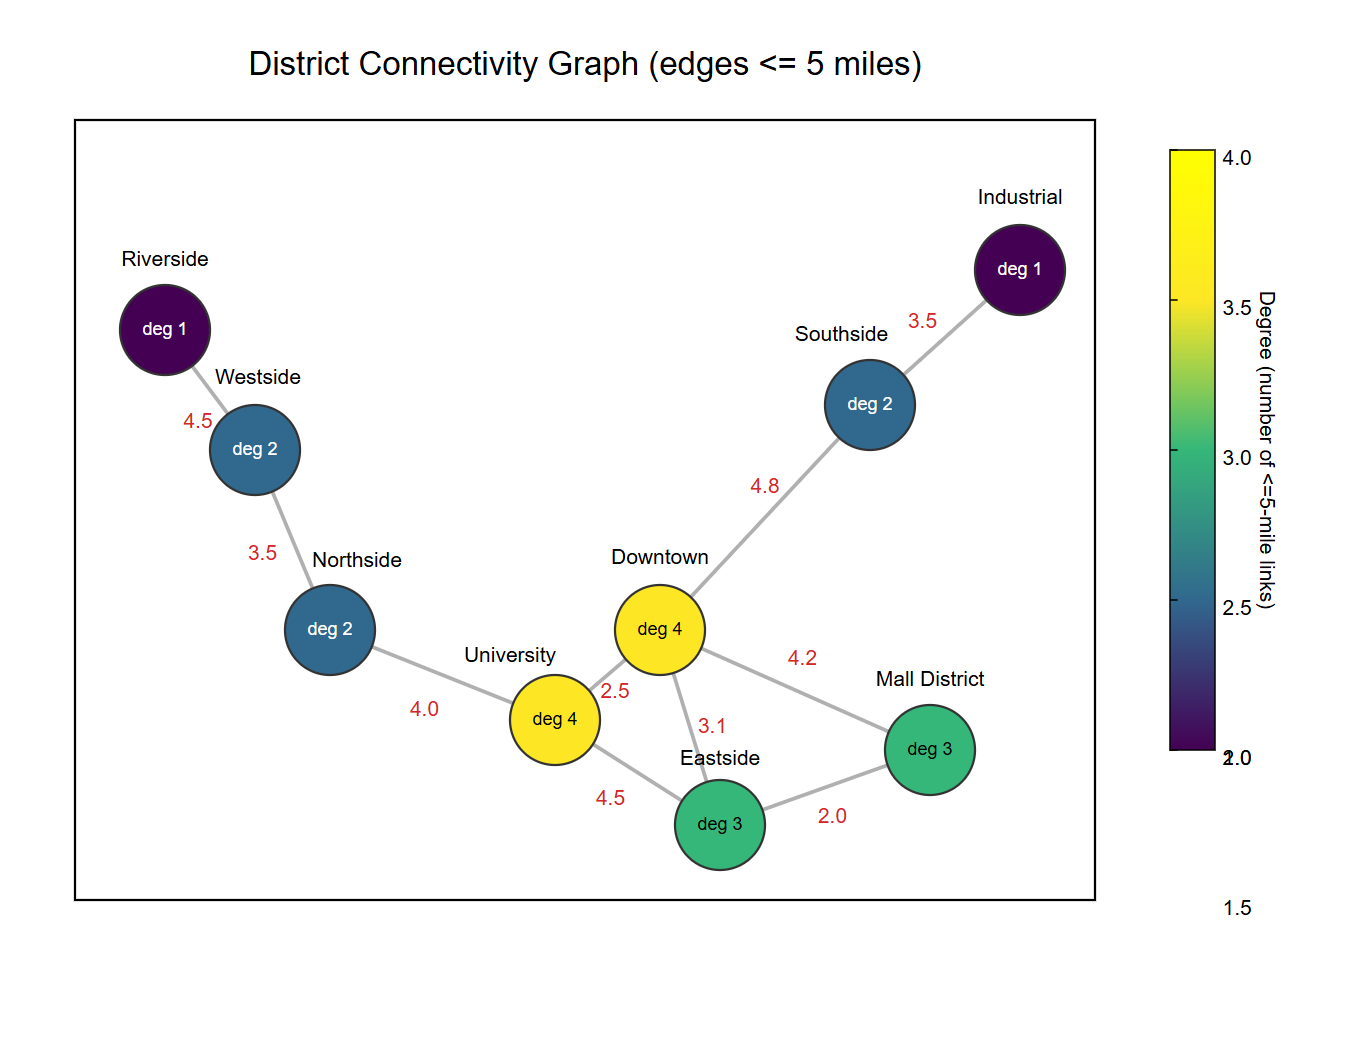
\includegraphics[width=0.65\textwidth]{ev_connectivity.png}
\caption{District connectivity graph with edges at distances of five miles or less.}
\label{fig:connect}
\end{figure}

Two findings emerge from the graph. First, it has exactly one connected component: every district is reachable from every other through a chain of five-mile hops, so the network is not fragmented and a central station can serve spillover demand from several neighbors. Second, the highest degree is four, held jointly by Downtown and University. A high-degree node is a natural hub with the most direct links, so a station there is accessible from the largest number of neighbors.

Downtown's hub status reinforces its Phase-1 selection, while University's equally high degree is informative precisely because it was not selected in Phase~1 despite its centrality. We now answer the problem's required comparison directly. Forcing University's site S7 into the Phase-1 set displaces S8 (Industrial) and raises the demand-weighted distance from 3.35 to 3.42 miles, a penalty of 2.12\%. Centrality alone does not override distance; a hub matters only when a station there also shortens the nearest drive for a high-demand district.

\subsection{Service and Financial Evaluation (Supplementary)}
\label{sec:service}

The $p$-median optimum is spatial. To verify that it is also operationally and financially sound, we evaluate each Phase-1 station using a steady-state M/M/c queue and the break-even formula introduced in Section~\ref{sec:breakeven}.

Each district is modeled as a first-come, first-served queue with $c_i$ ports. Arrivals are Poisson with peak rate determined by district EV count, service is exponential with mean one hour per vehicle, and the resulting utilization and mean waiting time follow the standard M/M/c relations:

\begin{equation}
\lambda_i = \frac{E_i}{70}, \qquad \rho_i = \frac{\lambda_i}{c_i \mu_i}, \qquad W_q^{(i)} = \frac{P_{\text{wait}}^{(i)}}{c_i \mu_i - \lambda_i},
\label{eq:queue}
\end{equation}

where $E_i$ is the district electric vehicle count, $\mu_i = 1$ vehicle per hour is the handling rate per port, $P_{\text{wait}}^{(i)}$ is the Erlang C probability that an arrival finds every port occupied, and the peak arrival rate $\lambda_i = E_i/70$ follows from Section~\ref{subsec:peak}. Equation~\eqref{eq:queue} is evaluated after Phase~1 opens, with the port count $c_i$ equal to existing ports plus newly installed ports in each district.

\begin{table}[H]
\centering
\caption{Service and financial evaluation of the Phase-1 sites.}
\label{tab:service}
\small
\begin{tabular}{llcccccc}
\toprule
Site & District & EVs (2024) & Ports after Phase 1 & $\lambda_{\text{peak}}$ & $\rho_{\text{peak}}$ & $W_q$ (min) & Break-even EVs \\
\midrule
S2 & Downtown   & 420 & 20 & 6.00 & 0.30 & $<$1 & 1{,}160 \\
S3 & Northside  & 310 &  9 & 4.43 & 0.49 &    3 &   960 \\
S4 & Southside  & 280 &  8 & 4.00 & 0.50 &    4 &   860 \\
S5 & Eastside   & 350 & 11 & 5.00 & 0.45 &    2 & 1{,}000 \\
S6 & Westside   & 290 &  5 & 4.14 & 0.83 &   43 &   740 \\
S8 & Industrial & 110 & 14 & 1.57 & 0.11 & $<$1 & 1{,}240 \\
\bottomrule
\end{tabular}
\end{table}

\begin{figure}[H]
\centering
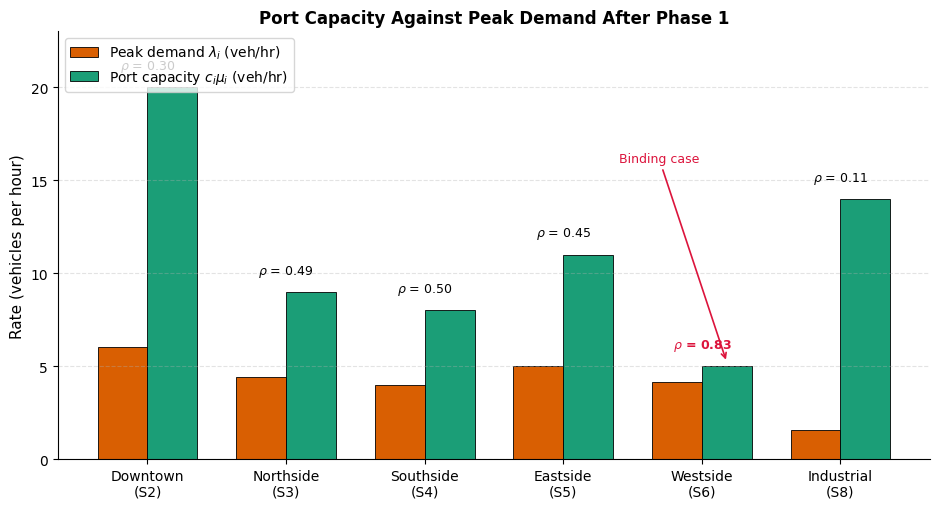
\includegraphics[width=0.75\textwidth]{ev_port_capacity.png}
\caption{Port capacity against peak demand after Phase 1.}
\label{fig:capacity}
\end{figure}

The results are informative. Five of the six Phase-1 stations operate comfortably below capacity. Westside is the binding case: with only five ports and 290 electric vehicles, peak utilization reaches 0.83 and mean waiting is approximately forty-three minutes. This is a clear argument for adding a second Westside station in Phase~2 or Phase~3, and it constitutes the strongest available justification for prioritizing Westside capacity expansion.

The Industrial site presents the opposite case. It is heavily underutilized at peak, with utilization of only 0.11, and it possesses the highest break-even count among the six selected sites, at 1,240 electric vehicles, against only 110 registered electric vehicles in Industrial today. It is therefore a coverage investment rather than a revenue-generating asset: it serves a peripheral district with no adjacent charger. Riverside, which has no chargers today, is not in Phase~1 but would score the highest service benefit per new port when it is added in Phase~3.

This evaluation does not change the Phase-1 selection, but it changes how the plan should be defended to the Council. The Industrial site is justified on coverage grounds rather than revenue, and Westside should be prioritized for capacity expansion in the second phase.

% ============================================================
\section{Task 3: Future Expansion Planning}
\label{sec:expansion}
% ============================================================

\subsection{Break-Even Analysis for Phase Timing}
\label{sec:breakeven}

The Phase-1 selection answers where to build first. To decide when to build the next stations, we require a data-driven trigger rather than an arbitrary electric vehicle threshold. We derive this trigger from a break-even calculation for each site. A station breaks even when the revenue it collects from the electric vehicles it serves covers its annualized cost. Amortizing installation over a ten-year horizon at $\alpha = 0.1$, and assuming each electric vehicle contributes fifty dollars per year in charging revenue, the break-even count of site $s$ is
\begin{equation}
\mathrm{BE}_s = \frac{0.1 c_s + m_s}{50}.
\end{equation}

\begin{table}[H]
\centering
\caption{Per-site break-even counts.}
\label{tab:breakeven}
\begin{tabular}{llccc}
\toprule
Site & District & Install cost & Annual maintenance & Break-even EVs \\
\midrule
S1  & Downtown      & \$450{,}000 & \$25{,}000 & 1{,}400 \\
S2  & Downtown      & \$380{,}000 & \$20{,}000 & 1{,}160 \\
S3  & Northside     & \$300{,}000 & \$18{,}000 &   960 \\
S4  & Southside     & \$280{,}000 & \$15{,}000 &   860 \\
S5  & Eastside      & \$320{,}000 & \$18{,}000 & 1{,}000 \\
S6  & Westside      & \$250{,}000 & \$12{,}000 &   740 \\
S7  & University    & \$350{,}000 & \$20{,}000 & 1{,}100 \\
S8  & Industrial    & \$400{,}000 & \$22{,}000 & 1{,}240 \\
S9  & Mall District & \$500{,}000 & \$30{,}000 & 1{,}600 \\
S10 & Riverside     & \$350{,}000 & \$18{,}000 & 1{,}060 \\
\bottomrule
\end{tabular}
\end{table}

A single site's break-even is a local condition. To time the phases citywide we use an empirical utilization rule: a public charger serves approximately seventy-five electric vehicles in comparable cities. We adopt seventy-five as a planning midpoint. A phase is justified once the chargers already deployed are serving seventy-five electric vehicles each on average. The city currently possesses thirty-three existing public chargers. Phase~1 adds forty chargers and brings the system total to seventy-three, so Phase~2 should begin when citywide electric vehicle registrations reach
\[
(41 + 40) \times 75 = 6{,}075\ \text{vehicles}.
\]
Phase~2 adds twenty chargers, raising the system total to ninety-three, so Phase~3 should begin at
\[
(41 + 40 + 20) \times 75 = 7{,}575\ \text{vehicles}.
\]
Under the ARIMA forecast, the city crosses 5{,}475 vehicles in 2027 and 6{,}975 vehicles in 2028. These crossing years establish the phase timing.

\subsection{Multi-Period Integer Program}

The $p$-median model answers where to build first. To answer what to build next, and in which year, we fix the Phase-1 layout and schedule the remaining sites with a discounted integer program. Let $x_{s,t} \in \{0,1\}$ indicate whether site $s$ is opened in phase $t \in \{2,3\}$. A site opened earlier serves demand sooner, so we discount phase-$t$ demand by $\delta^t$ with $\delta = 0.95$:
\begin{equation}
\max \sum_{t=2}^{3} \sum_{s \notin P_1} \delta^t q_s x_{s,t}
\end{equation}
subject to
\begin{gather}
\sum_{t=2}^{3} x_{s,t} \le 1 \quad \forall s, \\
\sum_{s \notin P_1} x_{s,t} = 2, \quad t = 2,3, \\
\sum_{s \notin P_1} c_s x_{s,t} \le 90, \\
x_{s,t} \in \{0,1\}.
\end{gather}
The quantity $q_s$ is the incremental demand weight of site $s$: the district's demand weight if the district has no station yet, and zero if it does. A second station in an already-served district, such as S1 in Downtown, adds no new coverage and therefore carries $q_s = 0$, deferring it to the last phase as a capacity site. The objective ranks the remaining coverage districts by discounted demand.

\begin{table}[H]
\centering
\caption{Optimal multi-period deployment.}
\label{tab:multiperiod}
\begin{tabular}{llccc}
\toprule
Phase & Sites opened & Stations & Cost & Weighted distance \\
\midrule
1 (2025--26) & S2, S3, S4, S5, S6, S8 & 6 & \$1{,}930{,}000 & 3.35 mi \\
2 (2027--28) & S7, S9                 & 2 & \$850{,}000     & 1.18 mi \\
3 (2029--30) & S1, S10                & 2 & \$800{,}000     & 0.00 mi \\
\midrule
\textbf{Total} & & \textbf{10} & \textbf{\$3{,}580{,}000} & \\
\bottomrule
\end{tabular}
\end{table}

The weighted-distance column carries the central message. Phase~1 reduces the demand-weighted distance from its unserved level to 3.35 miles. Phase~2, by giving the two remaining high-demand districts their own stations, reduces it further to 1.18 miles. Phase~3 eliminates it entirely, so that by 2030 every district has a station at zero distance.

\subsection{Three-Phase Deployment Roadmap}

The multi-period optimum, combined with the break-even crossing years, produces a three-phase roadmap. Phase~1 (2025--2026) constructs six stations at S2 (Downtown), S3 (Northside), S4 (Southside), S5 (Eastside), S6 (Westside), and S8 (Industrial), at a total cost of \$1.93 million, matching the $p$-median optimum of Section~\ref{subsec:phase1}. Phase~2 (2027--2028) adds S7 (University) and S9 (Mall District), triggered when citywide registrations cross 5{,}475 in 2027; University's degree-four centrality makes it an efficient second-wave hub. Phase~3 (2029--2030) adds S10 (Riverside), closing the city's only zero-charger district, and S1 as a second Downtown station, triggered when registrations cross 6{,}975 in 2028. By 2030 the forecast reaches 11{,}915 electric vehicles.

The roadmap is demand-driven at every step: the order of districts follows the demand ranking through the discounted objective, and the phase timing follows the break-even crossing years.

\subsection{Sensitivity Analysis}

We test how the plan responds to four classes of perturbation: electric vehicle growth error, installation-cost change, budget reduction, and forced station requirements.

When the electric vehicle growth forecast is scaled by $\pm 20\%$, the break-even crossing years shift by at most one year. The Phase-2 trigger of 5{,}475 vehicles moves between 2027 and 2028, and the Phase-3 trigger of 6{,}975 moves between 2028 and 2029. The order of district build-out is unchanged, because the demand weights feeding the $p$-median objective depend on relative differences that are stable under uniform scaling. The plan is robust in structure and only mildly sensitive in timing.

\begin{figure}[H]
\centering
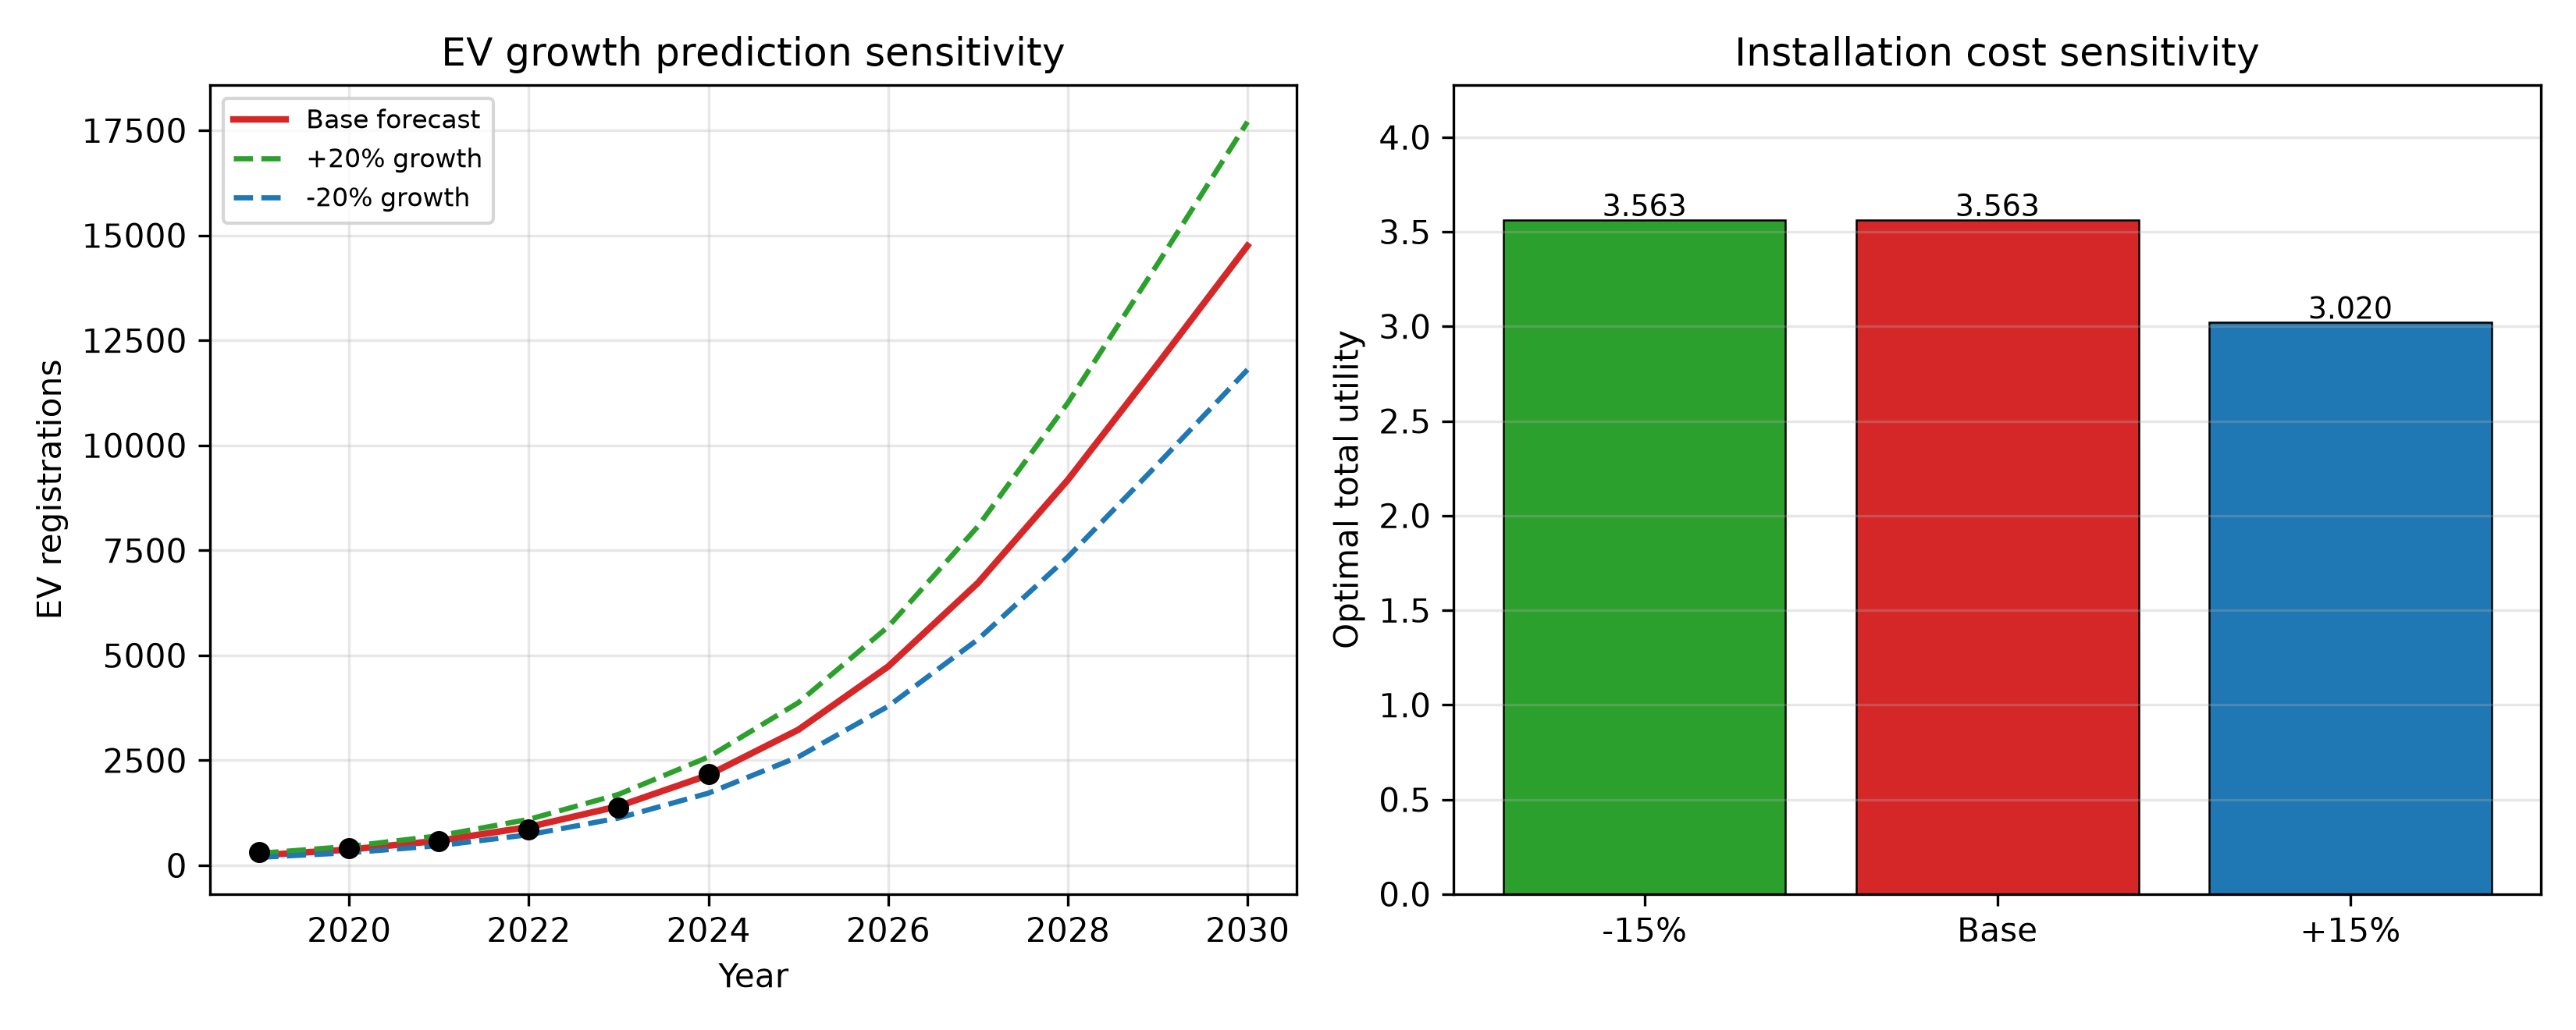
\includegraphics[width=0.8\textwidth]{ev_sensitivity.png}
\caption{Electric vehicle growth at $\pm 20\%$ shifts phase triggers by at most one year without altering the build order.}
\label{fig:sens}
\end{figure}

When installation costs are scaled by $\pm 15\%$, the optimum is unchanged at $-15\%$, with the six chosen stations retained and the demand-weighted distance holding at 3.35 miles. At $+15\%$, the budget binds, and the model drops S8 (Industrial), the station with the smallest marginal distance saving, settling on five stations at 4.59 miles. The plan is more sensitive to cost increases than to decreases, because the base plan already sits near the budget ceiling.

\begin{table}[H]
\centering
\caption{Optimal selection under installation-cost change.}
\label{tab:cost}
\begin{tabular}{llcc}
\toprule
Cost scenario & Selected sites & Stations & Weighted distance \\
\midrule
$-15\%$ & S2, S3, S4, S5, S6, S8 & 6 & 3.35 mi \\
Base   & S2, S3, S4, S5, S6, S8 & 6 & 3.35 mi \\
$+15\%$ & S2, S3, S4, S5, S6     & 5 & 4.59 mi \\
\bottomrule
\end{tabular}
\end{table}

Under successively tighter budgets, the core of Downtown, Eastside, and Westside persists across every scenario, confirming these as the highest-leverage locations. The marginal station is always Industrial (S8), which is the first to be dropped as the budget tightens and the last to return as it relaxes, consistent with its isolated-but-modest role in the spatial model.

\begin{figure}[H]
\centering
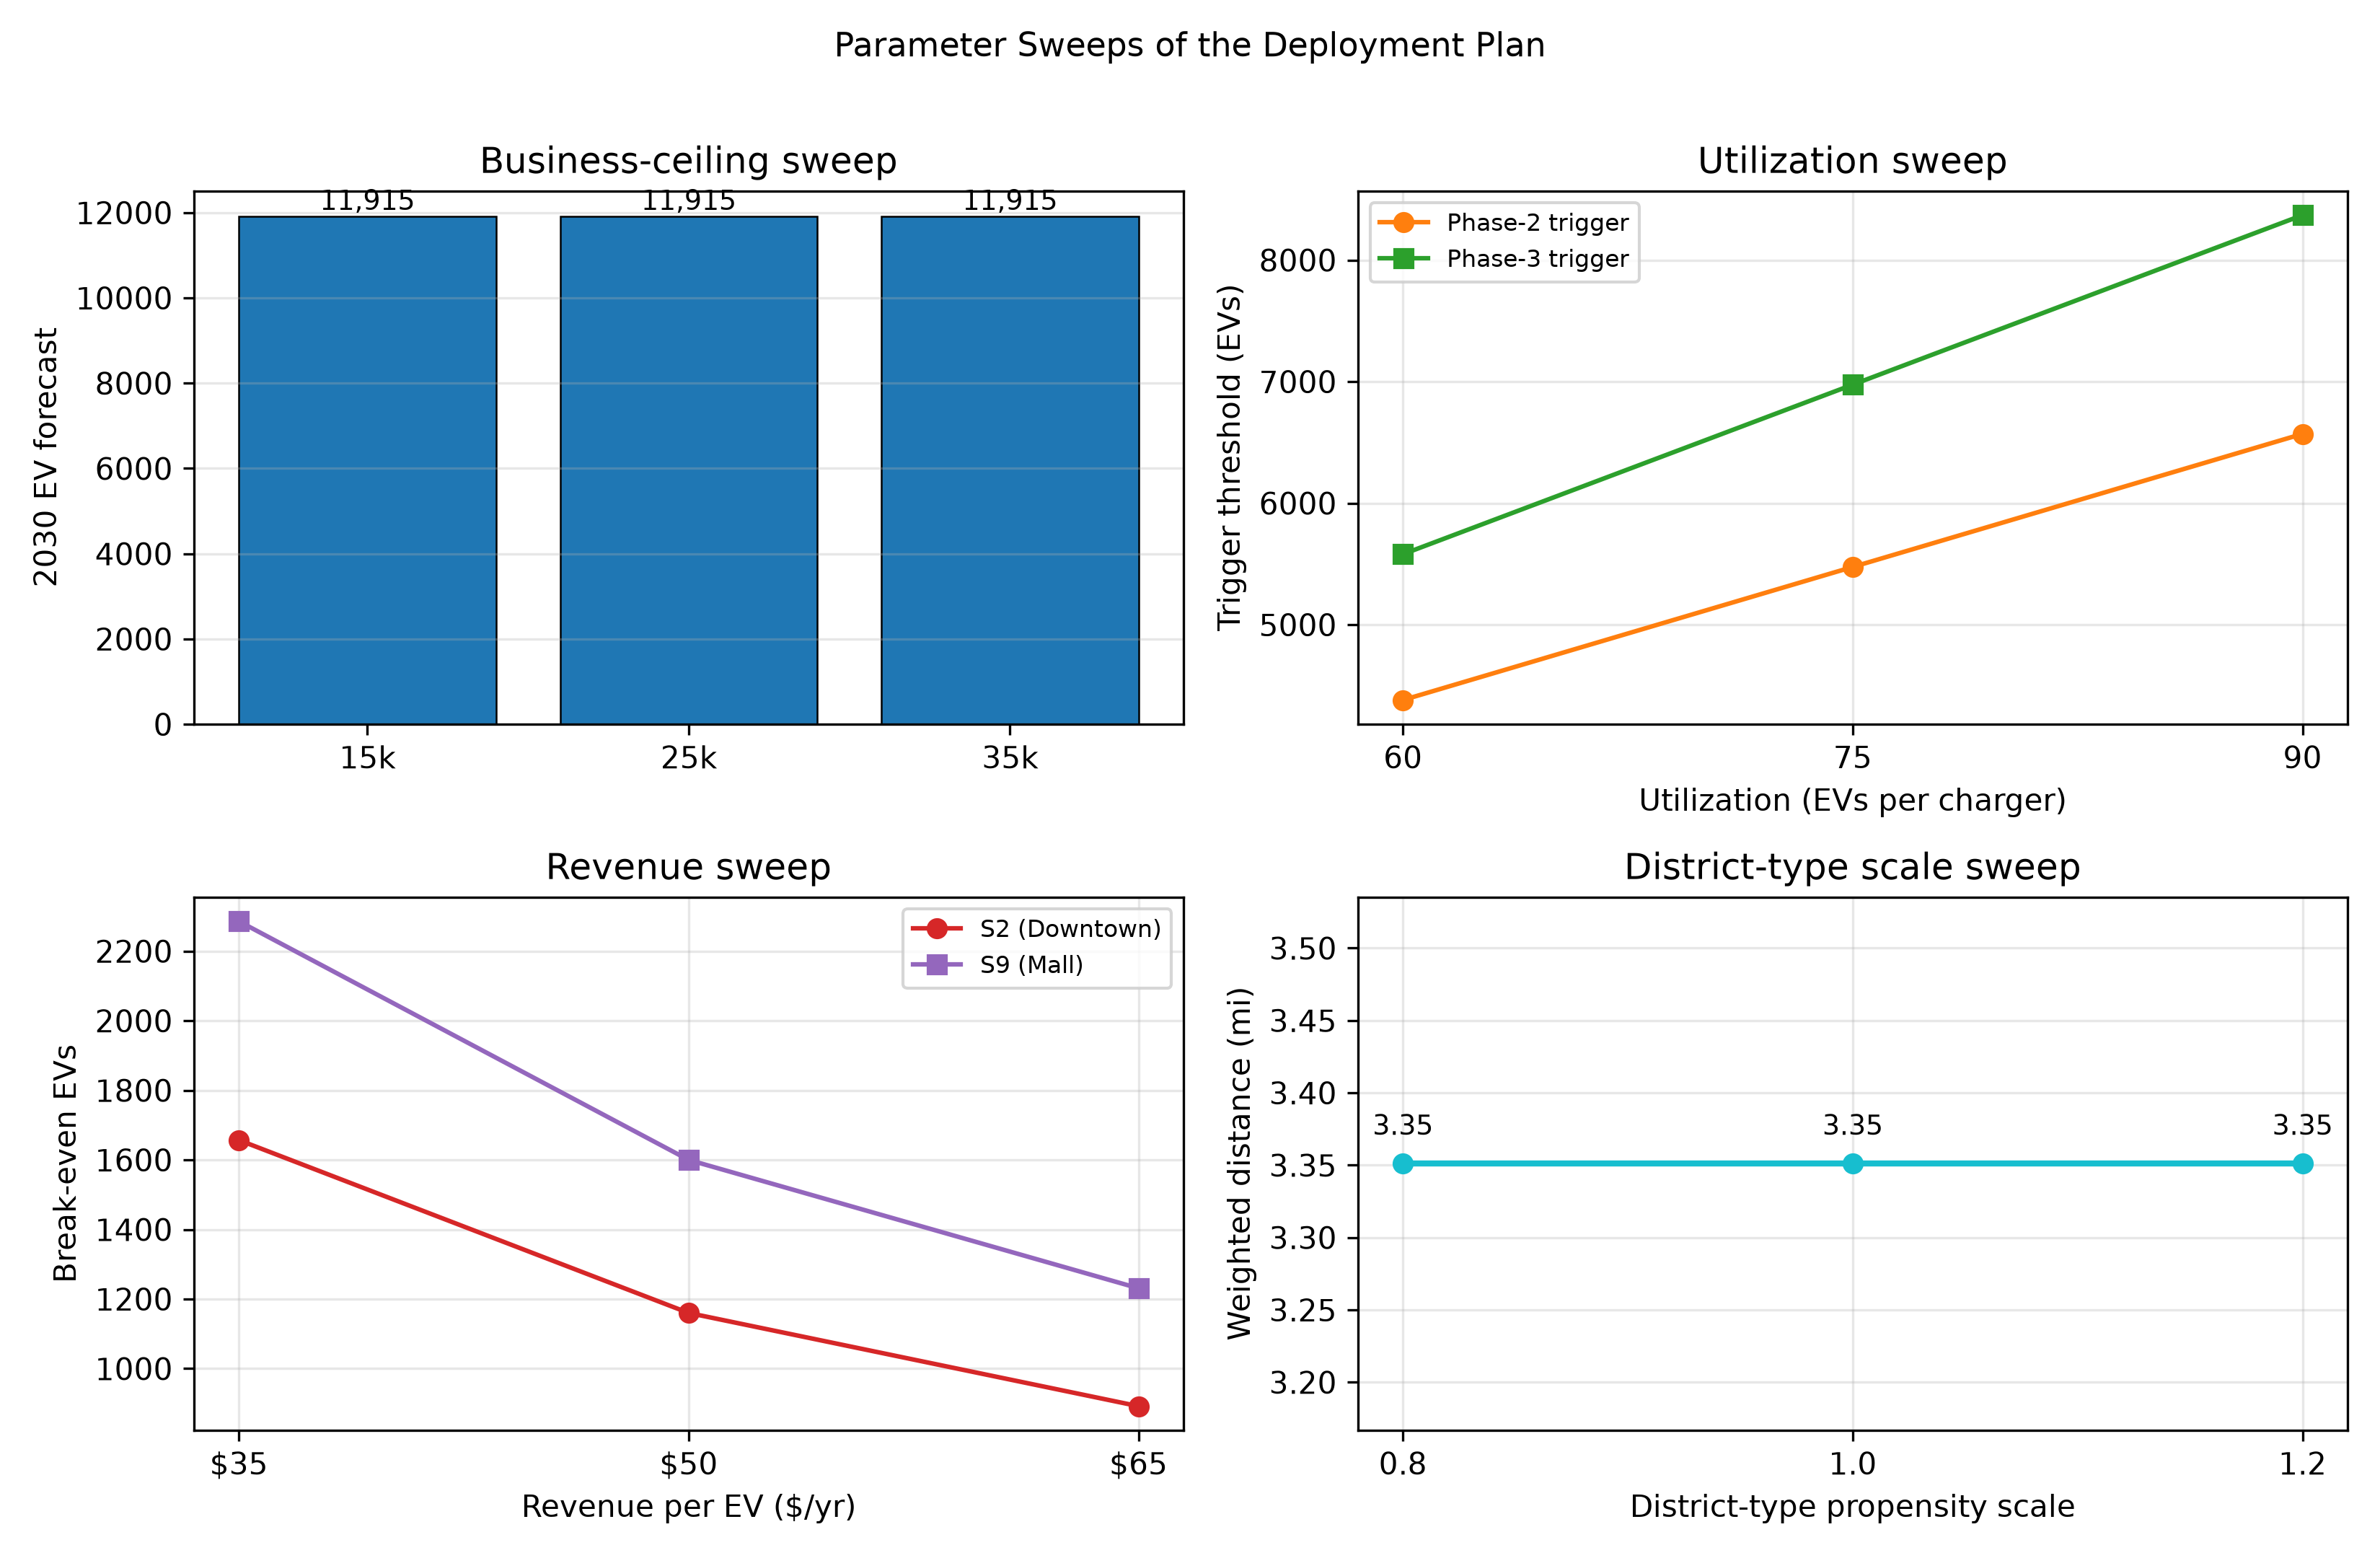
\includegraphics[width=0.5\textwidth]{ev_sensitivity_sweep.png}
\caption{Sensitivity sweep across budget, cost, and growth parameters.}
\label{fig:sweep}
\end{figure}

We also examine forced-station scenarios, in which the model is required to include a specific site regardless of cost. Forcing S7 or S10 into Phase~1 displaces S8 (Industrial), the most peripheral site, and raises the weighted distance from 3.35 to 3.42 miles, a penalty of approximately two percent. Both penalties are small, so the six-station core is not fragile. The penalties quantify the opportunity cost of departing from the distance-optimal selection.

\begin{table}[H]
\centering
\caption{What-if analysis under forced-station requirements.}
\label{tab:forced}
\begin{tabular}{llcc}
\toprule
Constraint & Selected sites & Distance & Penalty \\
\midrule
None (optimal)          & S2, S3, S4, S5, S6, S8  & 3.35 & --- \\
Must include University & S2, S3, S4, S5, S6, S7  & 3.42 & $+2.12\%$ \\
Must include Riverside  & S2, S3, S4, S5, S6, S10 & 3.42 & $+1.97\%$ \\
\bottomrule
\end{tabular}
\end{table}

Finally, we examine the sensitivity of the phase timing to the assumed revenue per electric vehicle. Doubling or halving the fifty-dollar benchmark shifts each site's break-even count proportionally, but the phase-timing thresholds of 5{,}475 and 6{,}975 vehicles are unaffected, because they depend on charger utilization rather than per-vehicle revenue. The overall deployment schedule is therefore insensitive to this parameter.

% ============================================================
\section{Model Evaluation}
\label{sec:Evaluation}
% ============================================================

\subsection{Strengths of the Model}

Our framework possesses several strengths that recommend it for practical deployment. First, the indicator weights are derived from the data through the entropy-weight method rather than imposed by expert judgment, which makes the demand ranking reproducible and free of subjective bias. Second, the location selections are provably optimal: because the candidate set is small, both the Phase-1 and multi-period programs are solved by complete enumeration, so the reported selections are globally optimal rather than heuristic approximations.

Third, the model is built around a single interpretable spatial objective. The $p$-median model minimizes one quantity, the demand-weighted travel distance, which possesses a direct physical meaning. Every chosen site is justified by the distance it saves for a high-demand district. Centrality and cost enter only as diagnostics and as a budget constraint, not as hidden trade-off coefficients. Fourth, the phase timing is data-driven: the break-even rule ties each build phase to a computed utilization threshold rather than an arbitrary electric vehicle count, and the multi-period program optimizes all phases jointly. Fifth, the supplementary M/M/c evaluation validates the spatial optimum against waiting time and financial viability, catching the Westside capacity shortfall and the Industrial coverage case that the spatial model alone would not expose. Finally, the entire pipeline executes in a fraction of a second, permitting interactive what-if analysis by city planners.

\subsection{Limitations and Avenues for Improvement}
\label{subsec:limitations}

We acknowledge several limitations. First, the ARIMA forecast is fit on only six annual observations, so the ADF test has limited power and the chosen model order is sensitive to the small sample. The 25{,}000-vehicle ceiling is a business judgment imposed after fitting rather than a fitted parameter. We have swept this ceiling over a wide range and confirmed that the near-term forecast is unchanged, but the limitation remains.

Second, the district-type propensity scale is a judgment-based mapping, though it is justified by the infrastructure literature. The Phase-1 selection is invariant to uniform rescaling of this scale because min-max normalization removes scale, but the relative ordering of district types still matters. Future work could replace the ordinal scale with measured proxies such as employment density or point-of-interest counts.

Third, the $p$-median model uses distance as a service proxy. It assumes that shorter distance is better but does not model waiting directly. The queue evaluation in Section~5.6 addresses this for the selected sites, but it is a post-selection check rather than an embedded constraint. A queuing-constrained location model would refine the analysis where demand is densest.

Fourth, the break-even analysis relies on a single revenue assumption of fifty dollars per electric vehicle per year. Real pricing and utilization data would refine the break-even counts, though we have verified that the phase-timing thresholds are insensitive to this parameter. Fifth, the queue evaluation treats each district as a closed local queue and does not model inter-district spillover; this is conservative and keeps the analysis tractable, but it understates the benefit of hubs in high-degree districts.

% ============================================================
\section{Conclusions}
% ============================================================

We have developed a quantitative framework for deploying Springfield's public electric vehicle charging network. Our primary contributions are as follows. We constructed a demand assessment model that scores the nine districts on six indicators using entropy weights and TOPSIS, producing a defensible ranking in which Downtown leads at 72.24 and Riverside trails at 26.11. We formulated and solved a $p$-median facility-location model that selects six Phase-1 stations at a total cost of \$1.93 million and a demand-weighted travel distance of 3.35 miles, optimal over every feasible six-site combination. We analyzed the connectivity of the district network and demonstrated that it forms a single connected component with Downtown and University tied for the highest degree.

We forecast electric vehicle registrations with an ARIMA$(1,2,0)$ model, projecting 3{,}242 vehicles in 2025, 6{,}083 in 2027, and 11{,}915 in 2030, and we used these forecasts to time a three-phase deployment roadmap that grows the network from six stations to ten and achieves full nine-district coverage by 2030. We supplemented the spatial model with an M/M/c queue evaluation demonstrating that five of the six Phase-1 stations reach break-even under the 2030 forecast and identifying the Industrial site as a coverage investment rather than a revenue-generating asset. Finally, we conducted a comprehensive sensitivity analysis demonstrating that the plan is stable under $\pm 20\%$ growth error and budget cuts, with only the marginal station at risk under a fifteen percent cost increase.

Future work could refine the queue evaluation to include inter-district spillover, replace the ordinal district-type scale with measured proxies, and embed queuing constraints directly in the location objective. The framework as presented transfers readily to any city that shares Springfield's data structure.

% ============================================================
% LETTER TO THE MAYOR
% ============================================================
\newpage
\section*{Letter to the Mayor and City Council}

\begin{center}
\emph{Mathematical Modeling Team \#10000}\\
\emph{Data Analytics Consultants to GreenCharge}\\
\emph{August 2026}
\end{center}

\noindent\textbf{To:} The Mayor and City Council of Springfield\\
\textbf{Subject:} A Plan for Springfield's Public Electric Vehicle Charging Network

\vspace{6pt}

We were asked three questions: where drivers need charging most, where the first stations should go, and how the network should grow. We write to present our answers.

What we found is that demand is concentrated. Downtown needs charging most, with the largest number of registered electric vehicles, the densest concentration of adoption, the busiest streets, and the highest concentration of businesses. Eastside is a clear second. Riverside occupies a special position: it has 120 registered electric vehicles and no public charger at all. Our forecast shows citywide registrations reaching approximately 6{,}100 by 2027 and 11{,}900 by 2030, which is why we recommend planning now rather than waiting for demand to arrive.

What we recommend is a three-phase build-out. In 2025 and 2026, we recommend constructing six stations in Downtown, Northside, Southside, Eastside, Westside, and Industrial, at a total cost of \$1.93 million. This is the set of stations that minimizes the average distance Springfield drivers must travel to reach a charger. In 2027 and 2028, we recommend adding two stations in the Mall District and University, timed to a break-even threshold that our forecast crosses in 2027. In 2029 and 2030, we recommend adding a station in Riverside and a second station in Downtown, so that every district has a charger and Riverside's gap is closed as its residents begin purchasing electric vehicles.

This plan is worth investing in for three reasons. First, it places chargers where they will actually be used, so the city does not pay for empty stations. Second, it is robust: if our growth forecast is off by twenty percent in either direction, the timing shifts by about a year but the order of construction holds; if installation costs rise by fifteen percent, the city builds five stations instead of six in the first wave. Third, we have verified that five of the six first-phase stations will cover their costs by 2030; the sixth, in Industrial, serves a district with no charger nearby and is justified on coverage rather than revenue grounds.

If we could do one thing to accelerate electrification, it would be to close Riverside's zero-charger gap sooner than currently scheduled. A driver with no charger in their district will not purchase an electric vehicle. One station there removes the single clearest barrier to adoption for an entire district, and we recommend the Council consider advancing it into the first phase.

We are happy to walk through the numbers behind each recommendation.

\vspace{8pt}
\noindent Respectfully submitted,\\
GreenCharge Data Analytics Team

% ============================================================
% REFERENCES
% ============================================================
\newpage
\begin{thebibliography}{99}

\bibitem{box2015}
G.~E.~P. Box, G.~M. Jenkins, G.~C. Reinsel, and G.~M. Ljung, \emph{Time Series Analysis: Forecasting and Control}, 5th ed. Hoboken, NJ: Wiley, 2015.

\bibitem{hyndman2018}
R.~J. Hyndman and G.~Athanasopoulos, \emph{Forecasting: Principles and Practice}, 2nd ed. Melbourne: OTexts, 2018.

\bibitem{dickey1979}
D.~A. Dickey and W.~A. Fuller, ``Distribution of the estimators for autoregressive time series with a unit root,'' \emph{Journal of the American Statistical Association}, vol.~74, no.~366, pp.~427--431, 1979.

\bibitem{shannon1948}
C.~E. Shannon, ``A mathematical theory of communication,'' \emph{Bell System Technical Journal}, vol.~27, pp.~379--423, 1948.

\bibitem{hwang1981}
C.~L. Hwang and K.~Yoon, \emph{Multiple Attribute Decision Making: Methods and Applications}. Berlin: Springer-Verlag, 1981.

\bibitem{daskin1995}
M.~S. Daskin, \emph{Network and Discrete Location: Models, Algorithms, and Applications}. New York: Wiley, 1995.

\bibitem{funke2019}
S.~Funke, F.~Sprei, T.~Gnann, and P.~Pl\"otz, ``How much charging infrastructure do electric vehicles need? A review of the evidence,'' \emph{Transportation Research Part D}, vol.~77, pp.~224--242, 2019.

\bibitem{doe2024}
U.S. Department of Energy, ``Alternative Fuels Data Center: Electric vehicle charging station locations,'' DOE AFDC, 2024.

\bibitem{iea2024}
International Energy Agency, ``Global EV Outlook 2024,'' IEA, Paris, 2024.

\bibitem{larson1981}
R.~C. Larson and A.~R. Odoni, \emph{Urban Operations Research}. Prentice-Hall, 1981, Ch.~4.

\bibitem{newman2010}
M.~Newman, \emph{Networks: An Introduction}. Oxford: Oxford University Press, 2010.

\end{thebibliography}

\newpage
\appendix
\section{Appendix: Python Implementation}
\label{app:code}

All numerical results in this paper are generated by a single Python program, \texttt{ev\_charging\_model.py}, provided as supplementary material. It depends only on standard scientific libraries and is deterministic or seeded, so every table and figure is exactly reproducible. Running \texttt{python3 ev\_charging\_model.py} regenerates all outputs in under a second.

The program is organized into modules that correspond to the paper's results.

\textbf{\texttt{data\_exploration()}} checks for missing values, computes $Z$-scores to flag outliers, and builds the indicator correlation matrix (Section~4.1).

\textbf{\texttt{demand\_model()}} normalizes the six indicators, derives entropy weights, and applies TOPSIS to produce demand scores (Tables~1--2).

\textbf{\texttt{arrival\_rates()}} converts district EV counts into peak and off-peak arrival rates using venue-type timing profiles (Section~4.6).

\textbf{\texttt{ev\_forecast\_arima()}} runs the ADF test, selects the ARIMA order by AIC, and forecasts registrations through 2030 with the 25{,}000-vehicle cap; \texttt{ev\_forecast()} fits the logistic baseline, and \texttt{compare\_forecasts()} prints the side-by-side table (Table~3, Figures~3--4).

\textbf{\texttt{location\_model()}} solves the $p$-median program of Section~5.2 by exhaustive enumeration over all 4--6 site combinations; \texttt{baseline\_comparison()} evaluates the demand-greedy, population-split, and random placement rules against the optimum (Tables~4--5).

\textbf{\texttt{graph\_model()}} builds the distance-threshold graph, computes node degrees, and finds connected components (Table~6, Figure~6).

\textbf{\texttt{queue\_evaluation()}} solves the M/M/c relations of Equation~\eqref{eq:queue} for each Phase-1 district, producing utilization and waiting time (Table~7, Figure~7).

\textbf{\texttt{break\_even()}} computes per-site break-even EV counts and the citywide phase-trigger thresholds (Table~8).

\textbf{\texttt{multi\_period()}} solves the discounted three-phase integer program with Phase~1 fixed (Table~9).

\textbf{\texttt{sensitivity()}} re-solves the location model under scaled growth, scaled costs, reduced budgets, and forced-station constraints, and sweeps the revenue assumption (Tables~10--11, Figures~8--9).

\end{document}